\documentclass[11pt,letter,fleqn,english,notitlepage]{article}
\usepackage{a4}
\usepackage{babel}
\usepackage{amsmath}
\usepackage{amssymb}
\usepackage{natbib}
\usepackage{setspace}
\usepackage{geometry}
\usepackage{graphicx}
\usepackage{eucal}
\usepackage{fancyhdr}
\usepackage{hyperref}
% \usepackage{url}
\usepackage{watermark}
\usepackage{listings}
%
\lhead[\fancyplain{}{\emph{A X I S E M}}] {\fancyplain{}{\emph{A X I S E M}}}
\chead[\fancyplain{}{}]                 {\fancyplain{}{}}
\rhead[\fancyplain{}{\emph{Tarje Nissen-Meyer}}]       {\fancyplain{}{\emph{Tarje Nissen-Meyer}}}
\lfoot[\fancyplain{}{}]                 {\fancyplain{}{}}
\cfoot[\fancyplain{}{\rightmark}]         {\fancyplain{}{\thepage}}
\rfoot[\fancyplain{} {}]  {\fancyplain{}{}}
%
\title{AXISEM 1.2 Manual}
\author{Tarje Nissen-Meyer, Martin van Driel, Simon Stähler, Kasra Hosseini}
%
\setlength{\topmargin}{-15mm}
\setlength{\textwidth}{165mm}
\setlength{\textheight}{220mm}
\hoffset=-5pt

%%%%%%%%%%%%%%  Newcommands paper3  %%%%%%%%%%%%%%%%%%%%
%
\newcommand{\eq}{\begin{equation}} \newcommand{\en}{\end{equation}}
\newcommand{\eqa}{\begin{eqnarray}} \newcommand{\ena}{\end{eqnarray}}
\newcommand{\subearth}{\raise.15ex\hbox{$\scriptstyle\oplus$}}
\newcommand{\Earth}{\raise.15ex\hbox{$\oplus$}}
\newcommand{\br}{\mbox{${\bf r}$}} \newcommand{\bs}{\mbox{${\bf s}$}}
\newcommand{\bu}{\mbox{${\bf u}$}} \newcommand{\bv}{\mbox{${\bf v}$}}
\newcommand{\bx}{\mbox{${\bf x}$}} \newcommand{\bw}{\mbox{${\bf w}$}}
\newcommand{\bC}{\mbox{${\bf C}$}} \newcommand{\bE}{\mbox{${\bf E}$}}
\newcommand{\bG}{\mbox{${\bf G}$}} \newcommand{\bI}{\mbox{${\bf I}$}}
\newcommand{\bM}{\mbox{${\bf M}$}} \newcommand{\bT}{\mbox{${\bf T}$}}
\newcommand{\bD}{\mbox{${\bf D}$}} \newcommand{\bU}{\mbox{${\bf U}$}}
\newcommand{\bK}{\mbox{${\bf K}$}} \newcommand{\bS}{\mbox{${\bf S}$}}
\newcommand{\bA}{\mbox{${\bf A}$}} \newcommand{\bQ}{\mbox{${\bf Q}$}}
\newcommand{\bF}{\mbox{${\bf F}$}} \newcommand{\bW}{\mbox{${\bf W}$}}
\newcommand{\bP}{\mbox{${\bf P}$}} \newcommand{\bB}{\mbox{${\bf B}$}}
\newcommand{\bR}{\mbox{${\bf R}$}} \newcommand{\bGamma}{\mbox{${\bf \Gamma}$}}
\newcommand{\bX}{\mbox{${\bf X}$}}
\newcommand{\rsubr}{\br_{\rm r}} \newcommand{\rsubs}{\br_{\rm s}}
\newcommand{\bzero}{\mbox{${\bf 0}$}}
\newcommand{\bdelta}{\mbox{\boldmath $\bf \delta$}}
\newcommand{\bPsi}{\mbox{\boldmath $\bf \Psi$}}
\newcommand{\bdel}{\mbox{\boldmath $\bf \nabla$}}
\newcommand{\bNcal}{\mbox{\boldmath $\bf {\mathcal N}$}}
\newcommand{\bFcal}{\mbox{\boldmath $\bf {\mathcal F}$}}
\newcommand{\bDcal}{\mbox{\boldmath $\bf {\mathcal D}$}}
\newcommand{\bsfM}{\mbox{\boldmath $\bf {\mathsf M}$}}
\newcommand{\bsfK}{\mbox{\boldmath $\bf {\mathsf K}$}}
\newcommand{\bsfU}{\mbox{\boldmath $\bf {\mathsf U}$}}
\newcommand{\bsfF}{\mbox{\boldmath $\bf {\mathsf F}$}}
\newcommand{\bsfp}{\mbox{\boldmath $\bf {\mathsf p}$}}
\newcommand{\bsfq}{\mbox{\boldmath $\bf {\mathsf q}$}}
\newcommand{\bsfu}{\mbox{\boldmath $\bf {\mathsf u}$}}
\newcommand{\bsfv}{\mbox{\boldmath $\bf {\mathsf v}$}}
\newcommand{\bsfw}{\mbox{\boldmath $\bf {\mathsf w}$}}
\newcommand{\bsff}{\mbox{\boldmath $\bf {\mathsf f}$}}
\newcommand{\bsfQ}{\mbox{\boldmath $\bf {\mathsf Q}$}}
\newcommand{\bsfW}{\mbox{\boldmath $\bf {\mathsf W}$}}
\newcommand{\bsfB}{\mbox{\boldmath $\bf {\mathsf B}$}}
\newcommand{\bsfI}{\mbox{\boldmath $\bf {\mathsf I}$}}
\newcommand{\bsfJ}{\mbox{\boldmath $\bf {\mathsf J}$}}
\newcommand{\bsfchi}{\mbox{\boldmath $\bf {\mathsf \chi}$}}
\newcommand{\bsfXi}{\mbox{\boldmath $\bf {\mathsf \Xi}$}}
\newcommand{\bsfYcal}{\mbox{\boldmath $\bf {\mathcal Y}$}}

\newcommand{\bsfzero}{\mbox{\boldmath $\bf {\mathsf 0}$}}
\newcommand{\bsfone}{\mbox{\boldmath $\bf {\mathsf 1}$}}
\newcommand{\sP}{\mbox{$\cal P$}} 
\newcommand{\sR}{\mbox{$\cal R$}}
\newcommand{\sS}{\mbox{$\cal S$}}
\newcommand{\bkh}{\mbox{$\hat{\mbox{${\bf k}$}}$}}
\newcommand{\blh}{\mbox{$\hat{\mbox{${\bf l}$}}$}}
\newcommand{\bnh}{\mbox{$\hat{\mbox{${\bf n}$}}$}}
\newcommand{\bph}{\mbox{$\hat{\mbox{${\bf p}$}}$}}
\newcommand{\brh}{\mbox{$\hat{\mbox{${\bf r}$}}$}}
\newcommand{\bsh}{\mbox{$\hat{\mbox{${\bf s}$}}$}}
\newcommand{\bth}{\mbox{$\hat{\mbox{${\bf t}$}}$}}
\newcommand{\bxh}{\mbox{$\hat{\mbox{${\bf x}$}}$}}
\newcommand{\byh}{\mbox{$\hat{\mbox{${\bf y}$}}$}}
\newcommand{\bzh}{\mbox{$\hat{\mbox{${\bf z}$}}$}}
\newcommand{\bthetah}{\mbox{$\hat{\mbox{\boldmath $\bf \theta$}}$}}
\newcommand{\bphih}{\mbox{$\hat{\mbox{\boldmath $\bf \phi$}}$}}
\newcommand{\bplh}{\mbox{$\hat{\mbox{\boldmath $\bf +$}}$}}
\newcommand{\bmih}{\mbox{$\hat{\mbox{\boldmath $\bf -$}}$}}
\newcommand{\ssR}{\mbox{${\sf R}$}} 
\newcommand{\sszero}{\mbox{${\sf0}$}} 

\newcommand{\uto}{\mbox{${\bf u}^{\hspace{-1.6ex}\raisebox{0.5ex}{$\scriptscriptstyle\rightarrow$}}$}} 
\newcommand{\vto}{\mbox{${\bf v}^{\hspace{-1.6ex}\raisebox{0.5ex}{$\scriptscriptstyle\rightarrow$}}$}} 
\newcommand{\vtos}{\mbox{${v}^{\hspace{-1.6ex}\raisebox{0.5ex}{$\scriptscriptstyle\rightarrow$}}$}} 
\newcommand{\Eto}{\mbox{${\bf E}^{\hspace{-1.6ex}\raisebox{1.0ex}{$\scriptscriptstyle\rightarrow$}}$}} 
\newcommand{\Tto}{\mbox{${\bf T}^{\hspace{-1.6ex}\raisebox{1.0ex}{$\scriptscriptstyle\rightarrow$}}$}} 
\newcommand{\Gto}{\mbox{${\bf G}^{\hspace{-1.6ex}\raisebox{1.0ex}{$\scriptscriptstyle\rightarrow$}}$}}
\newcommand{\ruto}{\mbox{${u}^{\hspace{-1.1ex}\raisebox{0.5ex}{$\scriptscriptstyle\rightarrow$}}$}}
\newcommand{\rvto}{\mbox{${v}^{\hspace{-1.1ex}\raisebox{0.5ex}{$\scriptscriptstyle\rightarrow$}}$}}
\newcommand{\rEto}{\mbox{${E}^{\hspace{-1.3ex}\raisebox{1.0ex}{$\scriptscriptstyle\rightarrow$}}$}}
\newcommand{\rTto}{\mbox{${T}^{\hspace{-1.4ex}\raisebox{1.0ex}{$\scriptscriptstyle\rightarrow$}}$}}
\newcommand{\svto}{\mbox{${\sf v}^{\hspace{-1.2ex}\raisebox{0.5ex}{$\scriptscriptstyle\rightarrow$}}$}} 
\newcommand{\sEto}{\mbox{${\sf E}^{\hspace{-1.3ex}\raisebox{1.0ex}{$\scriptscriptstyle\rightarrow$}}$}} 
\newcommand{\bAto}{\mbox{${\bf A}^{\hspace{-1.8ex}\raisebox{1.0ex}{$\scriptscriptstyle\rightarrow$}}$}} 
\newcommand{\Ato}{\mbox{${A}^{\hspace{-1.3ex}\raisebox{1.0ex}{$\scriptscriptstyle\rightarrow$}}$}}


\newcommand{\ufrom}{\mbox{${\bf u}^{\hspace{-1.6ex}\raisebox{0.5ex}{$\scriptscriptstyle\leftarrow$}}$}} 
\newcommand{\vfrom}{\mbox{${\bf v}^{\hspace{-1.6ex}\raisebox{0.5ex}{$\scriptscriptstyle\leftarrow$}}$}} 
\newcommand{\vfroms}{\mbox{${v}^{\hspace{-1.6ex}\raisebox{0.5ex}{$\scriptscriptstyle\leftarrow$}}$}} 
\newcommand{\Efrom}{\mbox{${\bf E}^{\hspace{-1.6ex}\raisebox{1.0ex}{$\scriptscriptstyle\leftarrow$}}$}} 
\newcommand{\Tfrom}{\mbox{${\bf T}^{\hspace{-1.6ex}\raisebox{1.0ex}{$\scriptscriptstyle\leftarrow$}}$}}
\newcommand{\rufrom}{\mbox{${u}^{\hspace{-1.1ex}\raisebox{0.5ex}{$\scriptscriptstyle\leftarrow$}}$}}
\newcommand{\rvfrom}{\mbox{${v}^{\hspace{-1.1ex}\raisebox{0.5ex}{$\scriptscriptstyle\leftarrow$}}$}}
\newcommand{\rEfrom}{\mbox{${E}^{\hspace{-1.3ex}\raisebox{1.0ex}{$\scriptscriptstyle\leftarrow$}}$}}
\newcommand{\rTfrom}{\mbox{${T}^{\hspace{-1.4ex}\raisebox{1.0ex}{$\scriptscriptstyle\leftarrow$}}$}} 
\newcommand{\svfrom}{\mbox{${\sf v}^{\hspace{-1.2ex}\raisebox{0.5ex}{$\scriptscriptstyle\leftarrow$}}$}} 
\newcommand{\sEfrom}{\mbox{${\sf E}^{\hspace{-1.3ex}\raisebox{1.0ex}{$\scriptscriptstyle\leftarrow$}}$}} 
\newcommand{\bAfrom}{\mbox{${\bf A}^{\hspace{-1.8ex}\raisebox{1.0ex}{$\scriptscriptstyle\leftarrow$}}$}}
\newcommand{\Afrom}{\mbox{${A}^{\hspace{-1.3ex}\raisebox{1.0ex}{$\scriptscriptstyle\leftarrow$}}$}} 

\newcommand{\bAboth}{\mbox{${\bf A}^{\hspace{-1.7ex}\raisebox{1.0ex}{$\scriptscriptstyle\leftrightarrow$}}$}}
\newcommand{\Aboth}{\mbox{${A}^{\hspace{-1.1ex}\raisebox{1.0ex}{$\scriptscriptstyle\leftrightarrow$}}$}}
%

%
\begin{document}
%
\pagestyle{fancy}
\thispagestyle{empty}
%
\begin{center}
{\LARGE {\sc AXISEM 1.2}}
\vspace{1.cm}\\
{\large 
Tarje Nissen-Meyer\textsuperscript{3)},
Martin van Driel\textsuperscript{2)},
Simon St\"{a}hler\textsuperscript{1)}
Kasra Hosseini\textsuperscript{1)}
} \\
{\small \textsuperscript{1)} LMU Munich, \textsuperscript{2)} ETH Zurich, 
\textsuperscript{3)} Oxford University \\
\vspace*{0.2cm}
\textit{tarje@alumni.princeton.edu} \hspace*{0.75cm}
\vspace*{0.5cm}\\ 
\today}
\end{center}
\thiswatermark{\begin{picture}(0,0) \put(-20,-190){\hspace{1.5cm}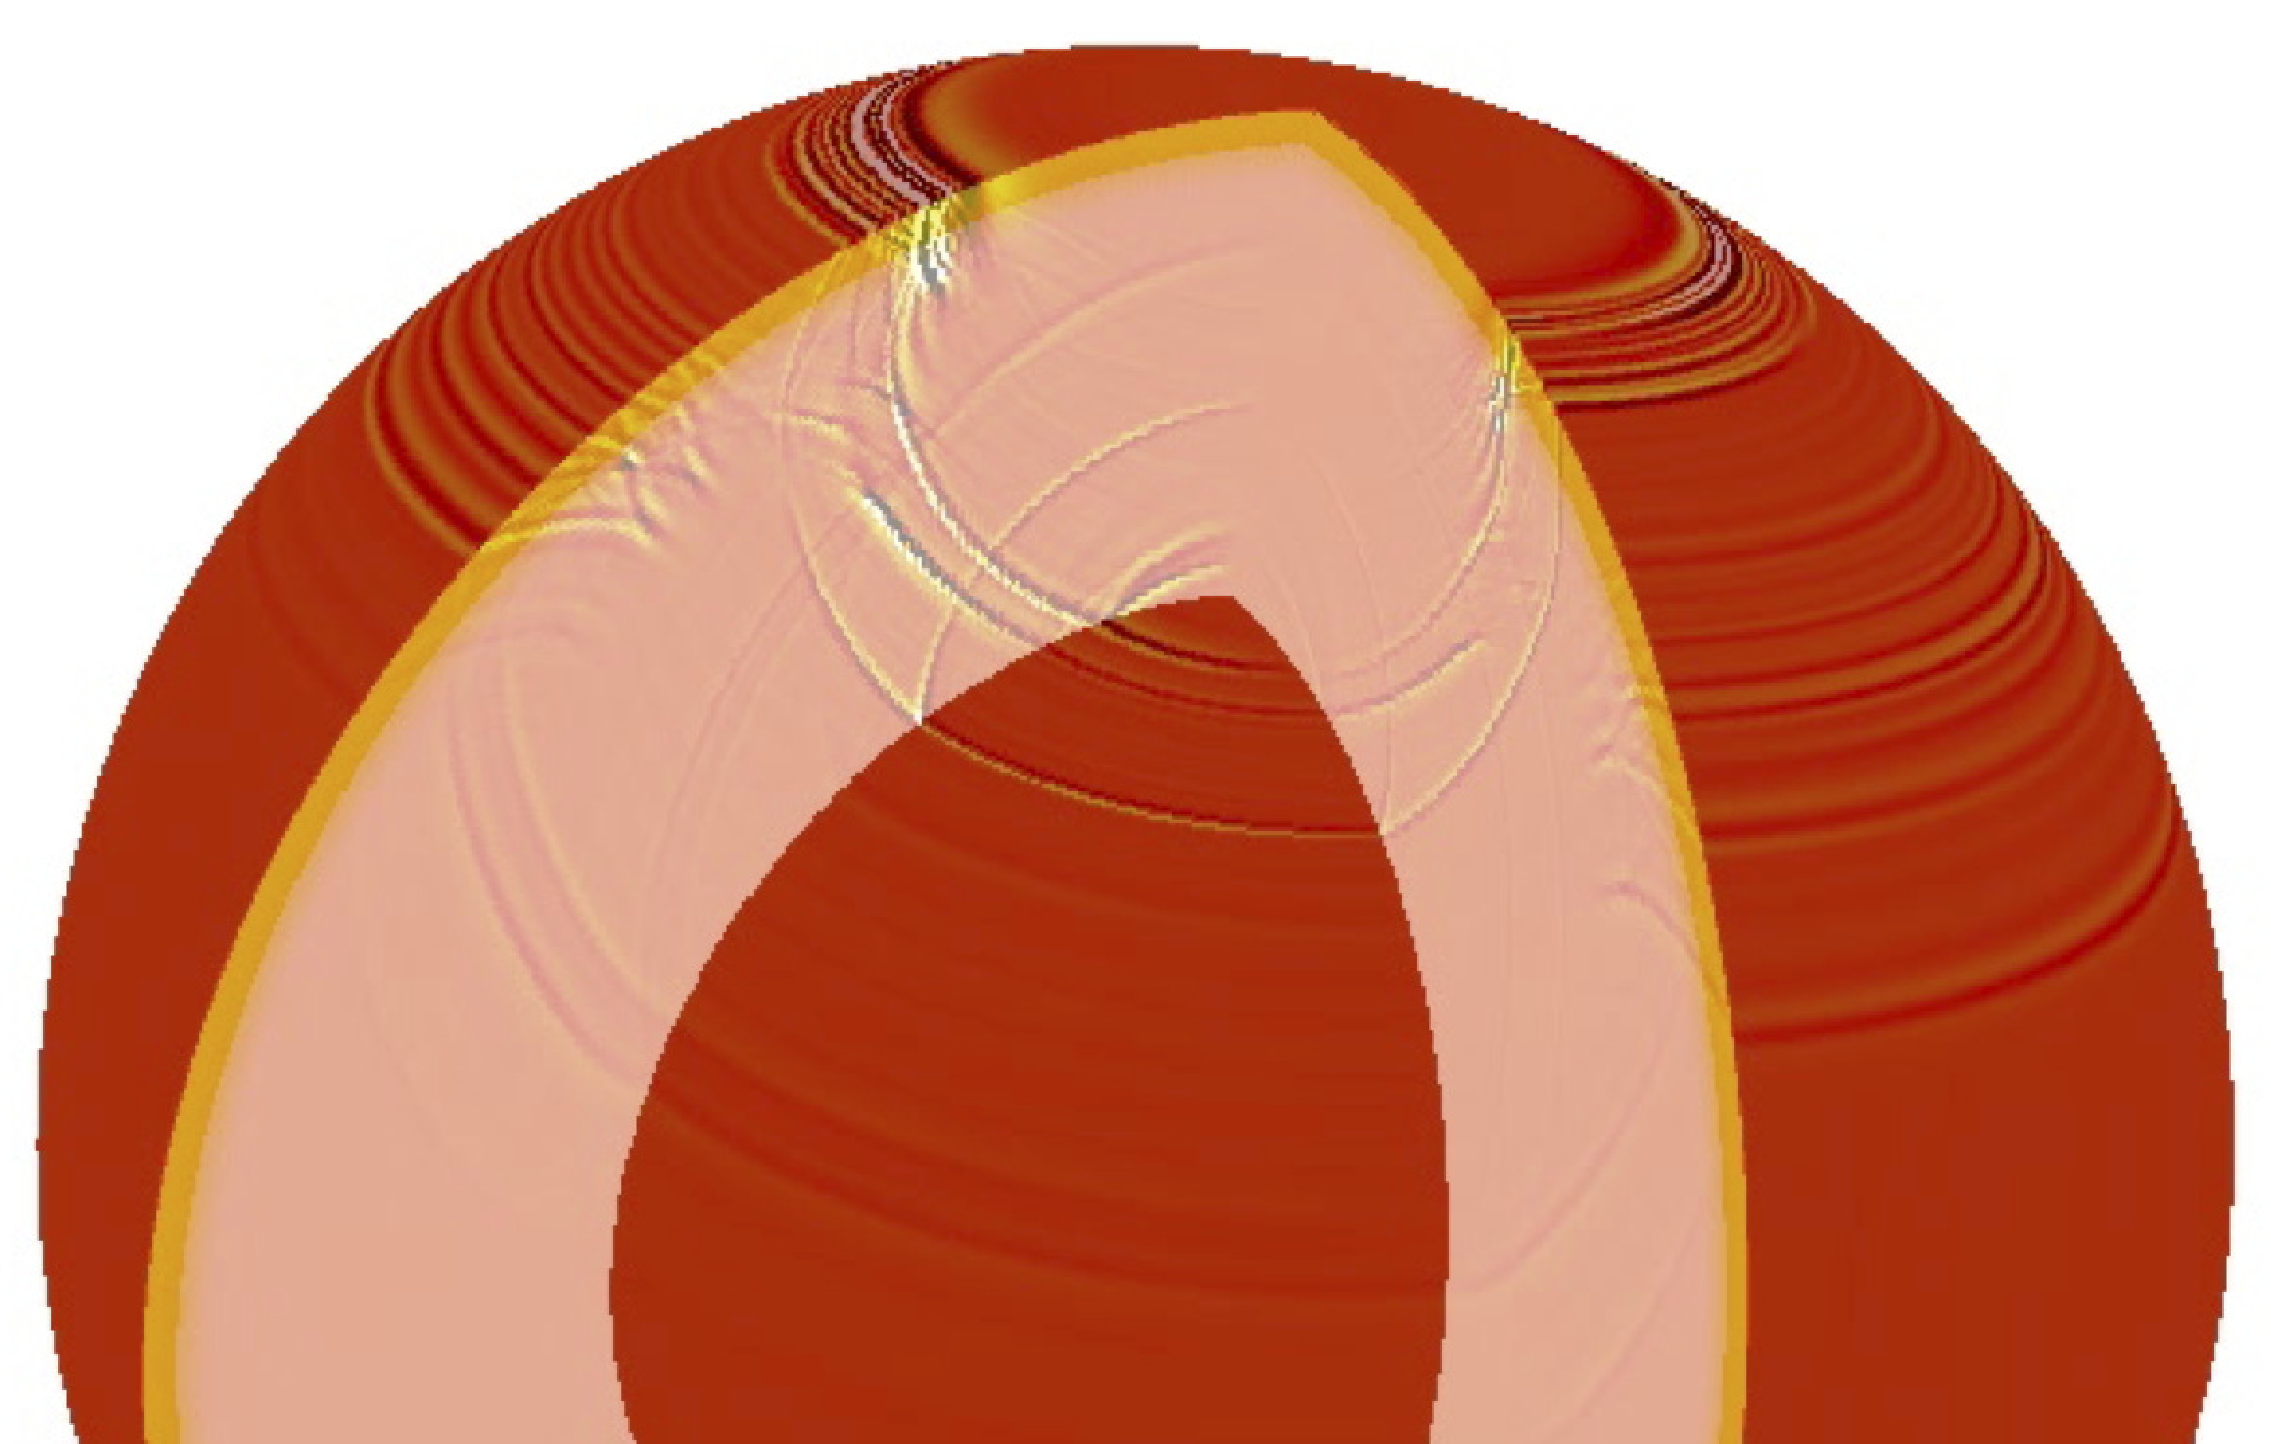
\includegraphics[width=0.9\linewidth]
{snap_cover_red.pdf}}\end{picture}}

\vspace*{1.6cm}
\noindent {\sc AXISEM} is a \textbf{parallel spectral-element method} to solve
3D wave propagation in a sphere with axisymmetric or spherically symmetric
visco-elastic, acoustic, anisotropic structures. Such media allow the
computational domain to be collapsed to a 2D disk, where the third, azimuthal
dimension is solved analytically on-the-fly posteriori. This leads to extreme
speedup by many orders of magnitude with respect to methods that discretize the
3D domain, and enables a full coverage of the seismic body- and surface wave
frequency spectrum between 0.001-1Hz.  The time-domain code delivers full
spatio-temporal wavefields that can be stored on disk and transformed to
frequency domain. Due to the dimensional reduction, global wave propagation at
typical seismic of \textbf{periods down to 5 seconds can be tackled on
laptops}, and at 1Hz on moderate clusters.

%Exploitation 
%of moment-tensor source and single-force radiation patterns allow the \textbf{computational domain 
%to be collapsed to a 2D semi-disk}, and the azimuthal third dimension is computed analytically.
%For each full earthquake moment tensor (single-force vector), 4 (2) simulations are undertaken that account for 
%tensor (vector) elements separately and are summed subsequently.
The Fortran 90 code is divided into a \textbf{Mesher}, a \textbf{Solver}
utilizing the message-passing interface (MPI) for communication between
separate domains, and \textbf{extensive post processing} for ease of
visualization.
%Radiation pattern symmetries require all sources 
%to be located along the axis, and any lateral heterogeneities are translated into a 2.5-dimensional
%ring-like structure.
The essential raison-d'\^{e}tre of this method is the \textbf{efficient
calculation of seismograms, wavefield movies, and those wavefields that underly
sensitivity kernels} to allow for tomographic inversions of any portion of a
seismogram at any relevant frequency. \\
%We have added methodological foundations directly extracted from the references.
%Eventually, we will add the sensitivity kernel software as well. \\

\noindent Provisional portal for this code at ETH Zurich:
\url{www.axisem.info}
%Please contact Tarje (\url{tarjen@ethz.ch}) for login information.

\section{Authors, contributors \& copyright}
%
\noindent \textbf{Principal authors:} Tarje Nissen-Meyer, Alexandre Fournier, Martin van Driel\\
\noindent \textbf{Contact:} Tarje Nissen-Meyer (\url{tarje@alumni.princeton.edu})\\
\noindent \textbf{Contributions:}
 J.-P. Ampuero, E. Chaljub, A. Colombi, F. A. Dahlen, S. Hempel, K. Hosseini, D. Komatitsch,
 G. Nolet, K. Sigloch, S. St\"{a}hler, J. Tromp.\\
\noindent \textbf{Research funding:} Princeton University, NSF (USA), SNF (Switzerland), 
the QUEST initial training network and ETH Zurich.\\
\noindent \textbf{Guarantees:} No guarantee whatsoever is given for this
software under any circumstances. It may be used freely for academic purposes
under the GNU license. Commercial use must be discussed with the authors prior
to usage.\\

\noindent \copyright  \hspace*{0.1cm} 
Copyright 2013, Tarje Nissen-Meyer (\url{tarje@alumni.princeton.edu}), Alexandre Fournier, Martin van Driel, Simon St\"{a}hler, Kasra Hosseini, Stefanie Hempel

AxiSEM is free software: you can redistribute it and/or modify it under the terms of the GNU General Public License as published by the Free Software Foundation, either version 3 of the License, or any later version.

AxiSEM is distributed in the hope that it will be useful, but WITHOUT ANY WARRANTY; without even the implied warranty of MERCHANTABILITY or FITNESS FOR A PARTICULAR PURPOSE.  See the GNU General Public License for more details.

A copy of the GPL can be found in the file \verb|LICENSE_GPL.txt|

\newpage
\tableofcontents
\newpage

\section{Preliminaries}

\subsection{Software and hardware requirements}

\subsubsection{Essential requirements:} 
\begin{description}
 \item[Compilers:] Fortran 90 compiler (tested on ifort, gfortran-4.6, portland)
 \item[Libraries:] MPI, NetCDF (optional)
 \item[Systems:] Unix-based OS (tested on Linux, MacOS, Cray XT4, XE6 and XK7)
 \item[Tools:] tcshell, perl
\end{description}
\subsubsection{Useful tools}
\begin{description}
 \item[ObsPy:] Needed for the automated tests. Follow the instructions for your system on \url{http://www.obspy.org}.
 \item[Paraview:] Can be used to check meshes and watch wavefield movies.
 \item[Google Earth:] Can be used for a quick overview on seismograms at the locations of the receivers.
 \item[gnuplot:] Used to make quick overview
\end{description}

% \textbf{Optional embedded software/libraries:} netcdf, python, taup, gnuplot

% \textbf{Optional processing software:} xmgr, matlab, paraview, google earth, obspy

% \subsection{Requirements}
% \textit{Basic requirements}: gfortran, MPI with gfortran support, tcshell, perl.
% \textit{Processing requirements (not obligatory)}: gnuplot, taup\\
% \textit{Visualization tools (suggested):} paraview, matlab, googleearth\\
 
\subsubsection{NetCDF}
AxiSEM allows to output larger datasets, especially wavefields in the NetCDF format. The current version also has full support for binary dumps, but the development will move towards NetCDF containers.\\
Unfortunately, the installation of the NetCDF libraries is not foolproof yet.
\begin{description}
 \item[HPC systems:] The libraries should be provided by the system. Use the recommended settings.
 \item[Ubuntu 12.10 and newer]: The code is working with the NetCDF libraries delivered with Ubuntu from version 12.10 (for gfortran). They can be installed by \\
 \verb|sudo apt-get install libnetcdff5|
 \item[Ubuntu 12.04 and older; MacOS]: The libraries delivered with Ubuntu 12.04 and earlier do not seem to work reliably. We therefore generally recommend to compile the NetCDF libraries from source. This can be done with the script \textit{make\_netcdf.sh} in the \verb|SOLVER/UTILS| directory. It downloads current versions of the zlib, hdf5 and netcdf4 libraries from \url{http://www.unidata.ucar.edu}, compiles them and runs the included tests. By default, the new libraries are installed in \verb|$(HOME)/local|. In the first lines of the script, specify your compiler (has to be the same as the one you are using for Axisem). The script should be run from a scratch directory like \verb|/tmp|:\\
 \verb|cd /tmp|\\
 \verb|$AXISEM_DIRECTORY/SOLVER/UTILS/make_netcdf.sh|\\
 Especially the HDF5 compilation will produce tons of warnings. They can be ignored, as long as the tests pass. If one of the tests should fail, the reason is most likely a wrong compiler configuration. We can offer only very limited support for the compilation of the libraries. 
 \item[Windows]: While we never tested it, installation of NetCDF on Windows should be possible:
 \url{http://www.unidata.ucar.edu/software/netcdf/docs/faq.html#windows_netcdf4_2}
\end{description}

\subsection{Preparation of a Debian/Ubuntu Linux system}
To prepare a fresh Debian-based Linux system, the absolutely necessary packages can be installed with:\\ \\
 \verb|sudo apt-get install gfortran build-essential tcsh openmpi-bin libopenmpi-dev|\\ \\
The processing and visualization tools can be installed with:\\ \\
 \verb|sudo apt-get install paraview gnuplot|

\section{Running the code}
\subsection{Quick start}
This is the step-by-step, blackbox procedure, i.e. running a workflow from raw source code to analyzing 
seismograms and wavefield movies upon pre-set parameters. It assumes your system fulfils all requirements mentioned above.\\
\begin{center}
\fbox{\parbox{0.65\textwidth}{
The default simulation parameters are: 
\begin{description}
 \item[PREM] velocity model (with anisotropy and anelasticity)
 \item[20 s] dominant period of the mesh
 \item[2 CPUs] used for the SOLVER
 \item[1800s] seismogram length
 \item[Wavefield movie] output enabled
 \item[Explosion] source
 \item[100 km] source depth
\end{description}
} }
\end{center}

\noindent Start from within the {\tt AXISEM} directory:

\begin{enumerate}
\item \verb|./copy_templates| $\Rightarrow$ creates various input files from templates
\item Check file \verb|make_axisem.macros|, whether the compiler settings fit your system.
\item \verb|cd MESHER| 
\item Check file {\tt inparamesh}, for background model, period of simulation and number of CPUs \\
      Default is \textit{PREM}, \textit{20 s} and \textit{2 CPUs} and runs within a few minutes on a modern PC.
\item \verb|./submit.csh| $\Rightarrow$ Check file {\tt OUTPUT}.
\item Wait for ``{\tt ....DONE WITH MESHER}'' to appear in {\tt OUTPUT}.
\item \verb|./movemesh.csh TEST_MESH| $\Rightarrow$ moves mesh files to \verb|../SOLVER/MESHES/TEST_MESH|.
\item \verb|cd ../SOLVER|
\item In \verb|inparam_basic| set the value for \verb|MESHNAME| to the meshname from above (e.g. \verb|TEST_MESH|)
\item \verb|./submit.csh TEST_SOLVER|  $\Rightarrow$ compiles and runs the code
\item \verb|cd TEST_SOLVER| $\Rightarrow$ Check \verb|OUTPUT_TEST_SOLVER|.
\item Wait for ``\verb|PROGRAM axisem FINISHED|'' to appear in \verb|OUTPUT_TEST_SOLVER| \\(use \verb|tail -f OUTPUT_TEST_SOLVER|).
\item \verb|./post_processing.csh|
\item \verb|cd Data_Postprocessing| 
\item \verb|googleearth|, open {\tt googleearth\_src\_rec\_processed.kml}, click
        earthquake (info), receivers (seismograms).
\item {\tt matlab}, run {\tt plot\_record\_section.m}, plotting all components
        of displacement seismograms.
% \item {\tt cd SNAPS; paraview}, load snaps for 3D wavefield movie.
% snaps are deacticated in defaulf...

\end{enumerate}
If the Solver is re-run with different parameters but the same mesh, you may start at step 9. 
To change model, frequency or number of CPUs, repeat steps 3. to 7. and select the new mesh in \verb|SOLVER/inparam_basic|. \\
The solver input can be changed in \verb|inparam_basic| between 8. and 9.,
changing post-processing input between 11. and 12. Using a new mesh requires
recompilation of the solver (done automatically in step 9.). If post
processing parameters are changed, also change the post processing directory or
delete the old one.

\subsection{Typical usecases}
\subsubsection{Change source type}
\verb|SOLVER/inparam_source|, \verb|SOLVER/CMTSOLUTION| and \verb|SOLVER/inparam_basic|.
Axisem has two principal modes, which are selected by the value \verb|SIMULATION_TYPE| in \verb|SOLVER/inparam_basic|.
\begin{enumerate}
 \item \verb|SIMULATION_TYPE single|:\\ The Solver simulates one basic source, which can be one of the following:\\
\begin{center}
\begin{tabular}{|l|cccc|} \hline
 monopoles:   & $M_{rr}$ & explosion  & $M_{\theta\theta}+M_{\phi\phi}$  & $P_r$ \\
 dipoles:     & $M_{\theta r}$ & $M_{\phi r}$        & $P_{\theta}$ & $P_{\phi}$\\
 quadrupoles: & $M_{\theta \phi}$ & $M_{\theta\theta}-M_{\phi\phi}$ & & \\\hline
\end{tabular}
\end{center}
where $M_{ii}$ are moment tensor sources with the mentioned components of $M$ set to one and the others to zero, $P_i$ is the same for single forces.\\
Choose the source type and set the source depth and amplitude in \verb|SOLVER/inparam_source|.
 \item \verb|SIMULATION_TYPE moment|:\\
 The submit.csh script starts four separate simulations for the basic types $M_{rr}$, $M_{\theta\theta}+M_{\phi\phi}$, $M_{\theta r}$, $M_{\theta \phi}$. You have to run the postprocessing script after the simulation to sum them up correctly. \\
 Before the simulation, set the source depth and the moment tensor in \verb|SOLVER/CMTSOLUTION|. Run \verb|postprocessing.csh| in the simulation directory afterwards. You can run postprocessing for different moment tensors on the same simulation, but not for different depths (since the forward simulation depends on the depth).\\
 The \verb|CMTSOLUTION| file is a standard format and can be downloaded from many sites in the web, including \url{http://www.globalcmt.org/CMTsearch.html}
\end{enumerate}



\subsubsection{Change station locations}
\verb|SOLVER/STATIONS| or \verb|SOLVER/receivers.dat|, depending on \verb|SOLVER/inparam_basic|, parameter \verb|RECFILE_TYPE|\\
\verb|SOLVER/STATIONS|: Similar to \textit{SPECFEM3D Globe}, an ASCII file with six columns, which are: station name, network name, latitude, longitude, elevation, depth (n.b: AxiSEM puts all receivers to the surface, the last two rows are ignored).
\begin{verbatim}
 RAYN   GD  23.52   45.50  0.0  0.0
 PALK   GD   7.27   80.70  0.0  0.0
 MAJO   GD  36.54  138.21  0.0  0.0
 ERM    GD  42.02  143.16  0.0  0.0
\end{verbatim}
The station names are used by post\_processing to assign names to the seismogram files.\\
\verb|SOLVER/receivers.dat|: Plain ASCII file with number of receivers in the first line and then nrec lines with colatitude and longitude.
\begin{verbatim}
 7
0.0 0.0
30.0 0.0
60.0 0.0
90.0 0.0
120.0 0.0
150.0 0.0
180.0 0.0
\end{verbatim}
\subsubsection{Change background model}
\verb|MESHER/inparam_mesh|, parameter \verb|BACKGROUND_MODEL|:\\
afterwards the steps from 5 have to be rerun. Supported models are
\begin{verbatim}
# prem_iso:               Isotropic continental PREM model
# prem_iso_solid:         like 'prem_iso', replace fluid outer core with vs=vp/sqrt(3)
# prem_iso_onecrust:      like 'prem_iso' but extend lower crust to surface
# prem_iso_light:         like 'prem_iso' but with mantle material extended to surface
# prem_iso_solid_light:   like 'prem_light', but in fluid outer core vs=vp/sqrt(3)
#
# prem_ani:               Anisotropic continental PREM model (actual PREM)
# prem_ani_onecrust:      like 'prem_ani' but extend lower crust to surface
# prem_ani_light:         like 'prem_ani' but with mantle material extended to surface
# 
# ak135                   AK135 (Isotropic, PREM attenuation)
# ak135f                  AK135 (Isotropic, own attenuation)
# iasp91:                 Isotropic IASP91 model with PREM density and attenuation
# external:               Layered external model, give file name in EXT_MODEL, the 
#                         inner core needs to be big enough, check VTK output.
\end{verbatim} 
\subsubsection{Change number of CPUs}
\verb|MESHER/inparam_mesh|, parameter \verb|NTHETA_SLICES| and \verb|NRADIAL_SLICES|: \\
The number of CPUs used is the product of the two parameters. \\
\verb|NTHETA_SLICES| needs to be 1, 2, 4 or a multiple of 4. To get a suggestion for optimal decomposition, run the Mesher with \verb|ONLY_SUGGEST_NTHETA true| and check the OUTPUT file.\\
\verb|NRADIAL_SLICES| should be less than 8. It can be left at 1 for \verb|NTHETA_SLICES|<64 CPUs, but should be increased then to reduce MPI communication.\\
N.B: This value is for ONE simulation. To calculate the wavefield of a full moment tensor, 4 parallel simulations have to be run and the number of necessary CPUs is \verb|NTHETA_SLICES|* \verb|NRADIAL_SLICES|*4. 
\subsubsection{Change the maximum frequency of the simulation}
\verb|MESHER/inparam_mesh|, parameter \verb|DOMINANT_PERIOD|: \\
As a rule of thumb: Simulations with \verb|DOMINANT_PERIOD|>10s can be run with 2 or 4 CPUs on a modern workstation and cost around 1 CPUh.
\subsubsection{Calculate the response to a full moment tensor solution}
\verb|SOLVER/inparam_basic|, change parameter \verb|SIMULATION_TYPE| to \verb|moment|:\\
The moment tensor, depth and location of the source must be set in the file \verb|CMTSOLUTION|. The submit.csh script starts four separate runs in parallel, the postprocessing script sums the results to get correct seismograms.
\subsubsection{Change seismogram length or sampling rate}
\verb|SOLVER/inparam_basic|, change parameter \verb|SEISMOGRAM_LENGTH|:\\
Default value is 1800~s, although the exact length is rounded to the next multiple of the simulation time step. There is no maximum limit, AxiSEM has been run for 400000s (5 days) to compare amplitude spectra with a normal modes summation.\\
\verb|SOLVER/inparam_advanced|, change parameter \verb|SAMPLING_RATE|:\\
By default, the sampling rate is set to the time step length of the simulation. We strongly recommend to leave it as such to avoid aliasing. The resampling can better be done with \textit{ObsPy} or another tool that supports filtering.

\subsubsection{Include lateral heterogeneities (2.5D simulation)}
\verb|SOLVER/inparam_basic|, change parameter \verb|LAT_HETEROGENEITY| to true:\\
The actual heterogeneity model is set in \verb|SOLVER/inparam_hetero|. 

% 
% \section{General remarks on the codes}
% 
% \textbf{Overview.} 
% 
% % TODO these 2 block are in large parts repetition of the introduction
% AXISEM is a parallel spectral-element method of the Gauss-Lobatto-Legendre type
% to solve the 3D solid-fluid equations of motion in a spherically symmetric
% sphere. The Fortran 90 source code is divided into a Mesher and a Solver
% utilizing the message-passing interface (MPI) for communication between
% separate domains. Due to symmetries in the earthquake radiation patterns, the
% 3D wavefield of an earthquake moment tensor is reconstructed from 4 separate
% simulations within a 2D computational domain. This D-shaped domain
% includes a non-physical boundary with singularities at the symmetry axis which
% is accomodated by Gauss-Lobatto-Jacobi discretization and l'Hospital's rule.
% Due to this symmetry, earthquake
% sources need to be located along this axis, and any lateral heterogeneities in
% the background model would be seen in an effectively ring-like structure.\\
% 
% The essential raison-d'\^{e}tre of this method is the efficient calculation of
% seismograms, wavefield movies, and specifically wavefields that constitute the
% crux for sensitivity kernels to allow for tomographic inversions of any portion
% of a seismogram at any relevant frequency. The two main parts are the mesher to
% construct a 2D domain for a given number of processors, resolution and input
% background model, and the solver which conducts the temporal evolution of the
% system explicitely at arbitrary spatial and up to sixth-order temporal
% accuracy.\\
% 
% 
% \subsection{General workflow}
% The generic workflow for both Mesher and Solver is as follows:
% \begin{enumerate}
% %    \item {\tt ./makemake.pl <arguments>}
% %    \item {\tt make clean; make}
%     \item Edit input parameters
%     \item {\tt ./submit.csh <arguments>}
% \end{enumerate}
% 
% %\noindent {\tt makemake.pl } generates the respective Makefiles. Argument \#1 options 
% %(check available options with {\tt ./makemake.pl -h}) include:
% %{\tt gfortran} and {\tt ifort}, argument \#2 is optional and only defined for
% %\tt debug}. Best is to try some options and check the Makefile to make sure it suits you.\\
% 
% \textbf{Input parameters: } Input ({\tt vi inparam\_mesh}) to the
% Mesher is simple, you should in most cases (of conventional earth models) not
% need to edit more than the first 3 parameters (earth model, seismic period, and
% number of processors).  Input to the Solver is attempted to be streamlined to
% the most primitive basis of settings as well. General input parameters are set
% in {\tt inparam\_basic}, more technical ones in {\tt inparam\_advanced}.  source and receiver parameters in separate files specified in {\tt inparam\_basic}).\\
% 
% {\tt submit.csh} are scripts to submit the jobs, check details with
% {\tt ./submit.csh -h} for both Mesher and Solver. In both cases, one can
% choose the queuing system (so far lsf, slurm and torque/maui) via arguments. 
% Note that in the case of a full moment tensor, 4 jobs will be submitted.
% % TODO: not implemented: , and in the case of a full force vector 2 (). 
% The script for the solver performs a variety
% of crucial operations for the simulations to succeed, act with sensitive care
% in case you really need to edit this script! \\
% 
% Upon successful completion of either job type, several
% post-processing options are available to indulge in. The mesher contains
% several vtk files to check the mesh via paraview, the solver contains a
% comprehensive and important series of operations invoked via {\tt
% ./post\_processing.csh } from the directory of the run. This includes summation
% over individual moment-tensor element responses, convolution with source time
% functions, rotation to actual source-receiver geometry, google-earth plots,
% seismograms in ascii and graphical formats, traveltime tables, 3D wave
% propagation snapshot movies, and a matlab script for plotting seismogram record
% sections.
% 
% \subsection{Algorithmic \& technical features}
% \begin{itemize}
%     \item Global numbering scheme (P. Fischer \& H. Tufo)
%     \item High-order symplectic time integration schemes (co-developed with Jean-Paul Ampuero)
%     % TODO: these are not well tested and give different results then newmark atm.
%     \item Unit-stride cache access, unrolled matrix products (Deville, Fischer, Mund)
%     \item Asynchronous (non-blocking) message passing (Tufo)
%     \item Output in VTK cell geometry
%     \item netcdf, xdmf file formats
%     \item python interface 
% \end{itemize}
% 
% \subsection{File formats}
% ???
% 
% \subsection{Automated testing}

This section is mainly useful for the develpers or those want to change/add/remove some parts of the code and compare the new changes with the reference solutions.
For the reference solutions, 5 different tests have been designed and 
the results from \textit{yspec} [Al-Attar \& Woodhouse (2008)] and AXISEM have been included in the \textit{TESTING/automatic} directory.
The whole procedure (running the code, compare the results and plot) is automatic with the least user intervention: \\

Start from within the {\tt AXISEM} directory:
 \begin{enumerate}
 \itemsep0em
 \item {\tt cd TESTING}
 \item {\tt python test\_axisem.py}
 \end{enumerate}

Enter test number(s) and this is all you should do! \\

\noindent As an example, we want to run the \textit{test\_axisem.py} for test number 5. (Figure~\ref{test_axisem})

\begin{figure*}[htb]
\begin{center}
\includegraphics[scale=0.4]{PYAXI/test_axisem.eps}
\caption{\textit{Screenshot while running test\_axisem.py}}
%\caption{\textit{}}
\end{center}
\label{test_axisem}
\end{figure*}

\noindent At the end, it plots three figures (one for each channel) 
in which the new AXISEM waveforms are compared with both the original ones and \textit{yspec} results for the same simulation.
%In Figure~\ref{channel_Z}, only the Z channel has been plotted.
It should be noted that these tests are designed for rough comparison purposes (in terms of the pulse shape and sign) and they should not be considered as a detailed benchmark with respect to YSPEC. \\

\begin{figure*}[htb]
\begin{center}
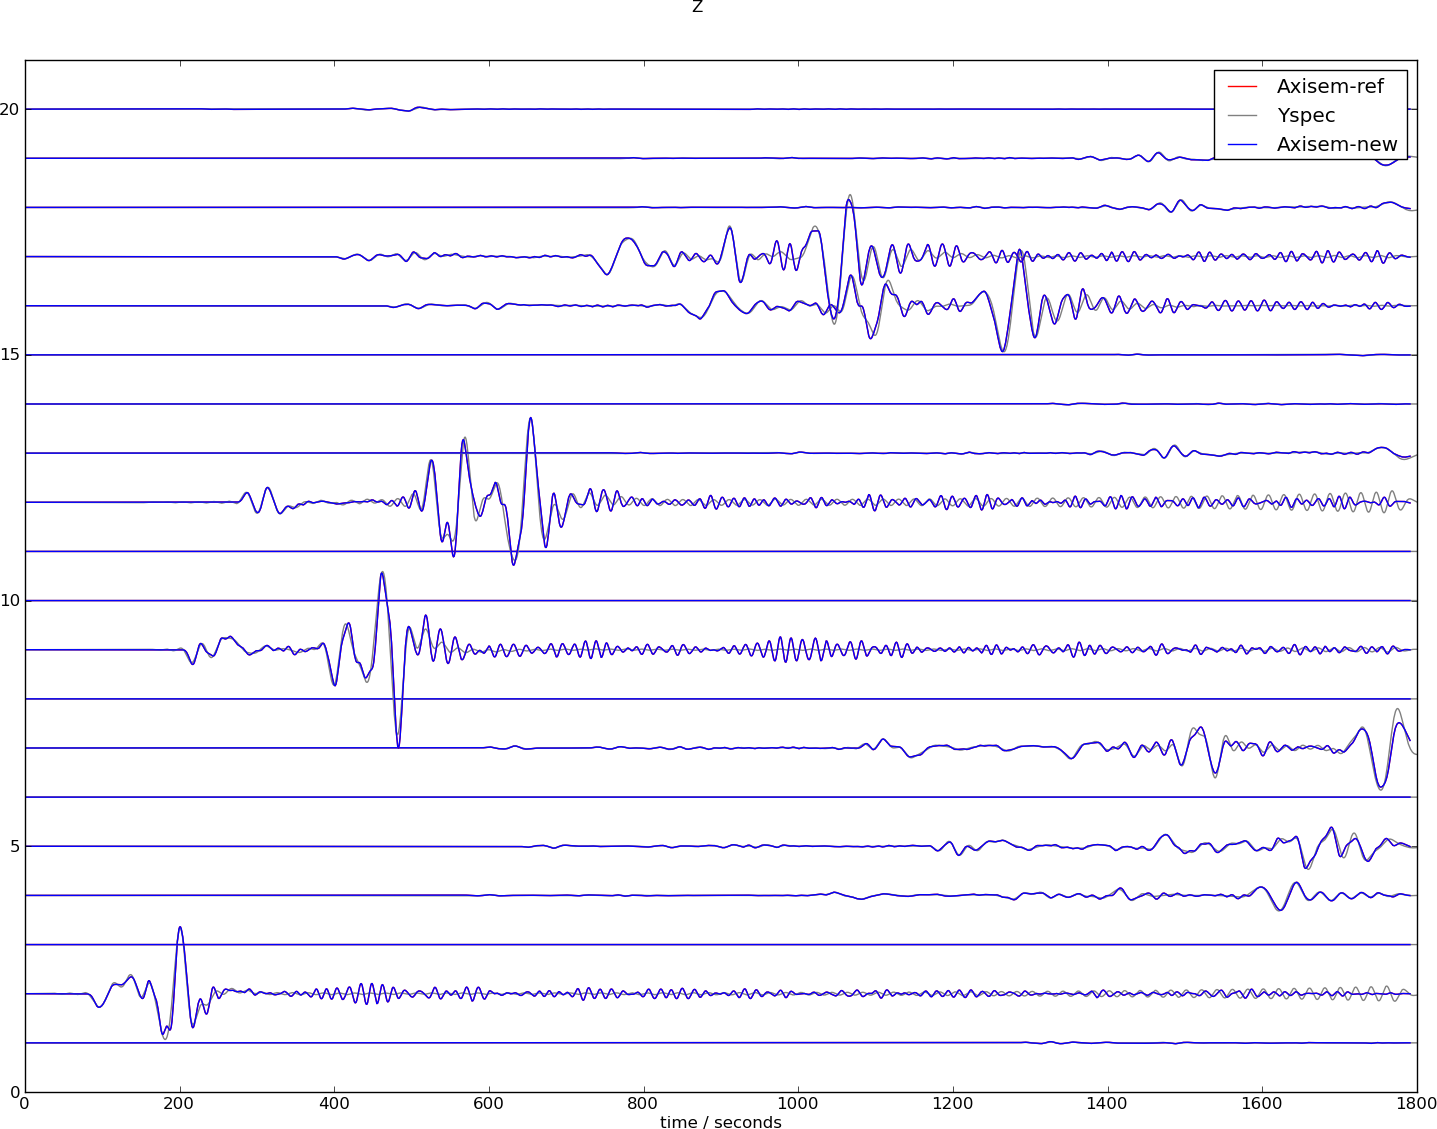
\includegraphics[scale=0.3]{PYAXI/record_section_Z.eps}
\caption{\textit{Comparing new AXISEM results with the reference solution and \textit{yspec} waveforms. (Z channel)}}
\end{center}
\label{channel_Z}
\end{figure*}

\noindent Another output is the \textit{l2} misfit (Figure~\ref{l2_misfit}) between the new and reference data 
in which the traces can be compared in a quantitative sense.

\begin{figure*}[htb]
\begin{center}
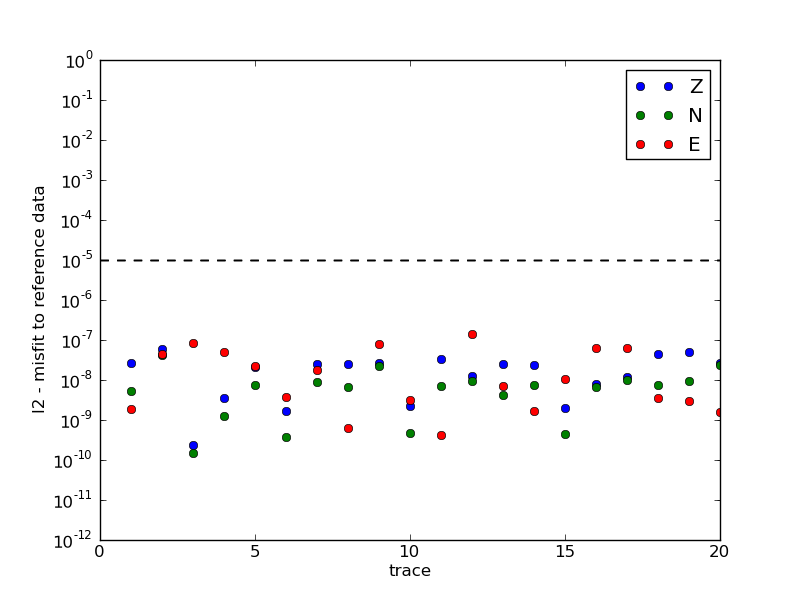
\includegraphics[width=0.8\textwidth]{PYAXI/l2_misfit.eps}
\caption{\textit{l2 misfit between the new and reference data.}}
\end{center}
\label{l2_misfit}
\end{figure*}

% 
% % \subsection{Virtual box: 3-hour tutorial}

COMMENTS: (with permission, I (Kasra) highlight the important parts for next references)

* Tarje:
Hi Kasra, on a quick look, this seems excellent, but from my experience it’s better to have a very easy and quick first run of the tasks, e.g. on ONE page with all the important calls and major points we wish to achieve... and delegate images and details to an appendix. So, let’s keep all this in but reshuffle it to have a concise early section. Tarje

I would structure it as I said in the email... pasting it here again:
Tutorial:
1) 10min intro
2) 10min big run (maybe drop this, depending on progress next week)
3) 60min virtual box: data and AxiSEM
4) 20min big run post processing
5) installation of AxiSEM, obspy locally

(TAS÷
1) Load data from one of the 5 events (Kasra) with Obspy, plot cross sections
2) change AxiSEM input parameters to run this scenario, submit job
3) check mesh, background model, source-receiver geometry (google earth)
4) run post processing, filter, sum, movie snapshots
5) Movie snapshots
6) plot data vs. synthetics
7) plot AxiSEM synthetics vs SPECFEM
8) change input parameters (source CMT), load run with different background model

The virtual box should therefore contain:
(DONE)        - all 5 events (metadata and data), each in one directory 
(PENDING) - AxiSEM source code structure (mesher, solver, manual, testing)
(DONE*)       - all axisem runs replicating the data for 2-3 background models and source choices
(PENDING)  - plots of seismograms, movie 
*: for each event there are: prem\_aniso and iasp91 for 5 (PENDING),10,50,100 seconds



AXISEM vs DATA:


Start from within the SCRIPTS directory:
1. python sta\_event\_plot.py ../EVENTS/EVENT-1: plot the event and all the stations in the selected directory (EVENT-1 in this example).
2. run AXISEM for one of these events. The required information is located in /EVENT-1/INFO.
3. 



































% 1. Introduction
% In this part of the tutorial, we want to compare AXISEM waveforms with real data. For this reason, three events are selected (Figure 1). Detailed information for each event can be found in APPENDIX-1.


% Figure 1: beach ball diagrams (based on GCMT catalog) of event-1 to event-3

% Figure-2 shows how these events and their meta-data are organized in the Virtual-box.

% ?????????????????SHOUDL BE ADDED?????????????????????
% Figure 2: folder structure

% In SCRIPTS directory, two python scripts are provided that we will use here:
% 1. epi_plot.py: plotting tool for comparison purposes.
% 2. tt_plot.py: project the time shift derived by cross correlating the AXISEM waveforms and real data.

% 2. Run AXISEM
% As the first step, we want to simulate event-2 (Figure-3) with AXISEM. All the required AXISEM input files are provided in ????folder???.  APPENDIX-2 gives a quick overview on how to run AXISEM using PyAxi (Python interface for AXISEM).

% Figure 3: event and station configuration for event-2

% Once your simulation is done, all the AXISEM synthetic waveforms should be moved to ????folder???:
% cp <synthetic_waveforms> <destination????>

% 3. Compare the results
% To have an idea on how the synthetic and real data look like:
% python epi_plot.py ????address???


% Figure 4: AXISEM and real data waveforms arranged by epicentral distance

% For one specific seismic phase (Pdiff in this example), the following command plots the results of AXISEM against the real data: (to change the frequency?????)
% python epi_plot.py ../EVENTS/EVENT-2/AXISEM_PRE_SIMULATED/PREM\_ANISO_5sec/ Pdiff

% Figure 5: AXISEM and real data waveforms arranged by epicentral distance (Pdiff seismic phase)

% SPECFEM3D waveforms can be also added to the comparison by: (how to retrieve SPECFEM?!?!?!?!?)
% python epi_plot.py ../EVENTS/EVENT-2/AXISEM_PRE_SIMULATED/PREM_ANISO\_5sec/ Pdiff specfem3D
% Figure 6: AXISEM, SPECFEM3D and real data waveforms arranged by epicentral distance (Pdiff seismic phase)


% 4. Travel time measurements
% The time shift between AXISEM and real data (Figure 5) can be roughly measured by cross-correlating the time series. epi_plot.py can perform this and shift the synthetics in order to match them up:
% python epi_plot.py ../EVENTS/EVENT-2/AXISEM_PRE_SIMULATED/PREM_ANISO_5sec/ Pdiff shift_synthetics

% Figure 7: AXISEM and real data waveforms arranged by epicentral distance (Pdiff seismic phase), synthetic waveforms are shifted based on cross-correlation analysis.

% The calculated time shift can be mapped on the relevant station for the selected phase:
% python tt_plot.py ../EVENTS/EVENT-2/

% APPENDIX-1: Events
% ????????

% APPENDIX-2: A Quick Guide to PyAxi
% PyAxi (Python interface for AXISEM) is a Python script to run AXISEM automatically.

% python PyAxi <inpython.cfg> <STATIONS>

% and the rest should be done automatically. Therefore, to run the AXISEM for the provided examples (I mean! AXISEM_pre_simulated), it is enough to run:


% APPENDIX-3: Retrieving SPECFEM3D seismograms


% Event-1:
% ./obspyDMT.py --datapath EVENT-1 --min_date 2009-07-15 --max_date 2009-07-16 --min_depth 20 --list_stas /home/hosseini/Desktop/ALASKA_VBOX_LATEST/EVENTS/EVENT-1/INFO/STATIONS --specfem3D --offset 3600 --min_mag 7.0 --req_parallel --arc N

% Event-2:
% ./obspyDMT.py --datapath EVENT-2 --min_date 2009-09-30 --max_date 2009-10-01 --min_depth 70 --list_stas /home/hosseini/Desktop/ALASKA_VBOX_LATEST/EVENTS/EVENT-2/INFO/STATIONS --specfem3D --offset 3600 --min_mag 7.0 --req_parallel --arc N

% Event-3:
% ./obspyDMT.py --datapath EVENT-3 --min_date 2006-10-15 --max_date 2006-10-16 --min_depth 20 --list_stas /home/hosseini/Desktop/ALASKA_VBOX_LATEST/EVENTS/EVENT-3/INFO/STATIONS --specfem3D --offset 3600 --min_mag 6.0 --req_parallel --arc N

% % seperate document by now
% 
% \subsection{PyAxi: Python interface for AXISEM}

\subsection{Introduction}
PyAxi is a Python script developed as an interface for AXISEM. 
All the options available in AXISEM are included in only one input file (\textit{inpython.cfg}).
By running the script, all the necessary steps (MESHER, SOLVER and Post-Processing) will be done automatically.
Python is the only requirement; However, some special functionalities (mseed format, plotting in Python environment) need \textit{ObsPy} to be installed. \\

\noindent \textit{Basic requirement}: Python.\\
\textit{Convert to MSEED (not obligatory)}: ObsPy (https://github.com/obspy/obspy/wiki).\\

\subsubsection{How to Run PyAxi?}
%In this part, we show how to run PyAxi for different input files.
First, let's check whether AXISEM can be run properly on our machine. 
For this reason:\\

Start from within the {\tt AXISEM} directory:
\begin{enumerate}
\itemsep0em
\item {\tt cd TESTING}
\item {\tt python PyAxi.py --check}
\end{enumerate}
\noindent This gives an overview of the installation status of all relevant compilers and tools required
to run AXISEM on your machine (Figure~\ref{check_pyaxi}). 
Please note that \textit{--check} does not check for all the possible compilers.
It just checks for those listed in Figure~\ref{check_pyaxi}; 
therefore, for other compilers, it should be done manually.\\

\begin{figure*}[htb]
\begin{center}
\includegraphics[scale=0.32]{PYAXI/check_pyaxi.eps}
%\caption{\textit{}}
\end{center}
\caption{\textit{Checking all the relevant compilers and tools required to run AXISEM.}}
\label{check_pyaxi}
\end{figure*}


\noindent After installation of all required packages, 
maybe the best way to get familiar with AXISEM is to run the code with the default input file:\\

Start from within the {\tt AXISEM} directory:
\begin{enumerate}
\itemsep0em
\item {\tt cd TESTING}
\item {\tt python PyAxi.py inpython.cfg}
\end{enumerate}

All the rest will be done automatically...\\

\noindent \textit{inpython.cfg} is a configuration file that contains all the AXISEM options.
To change the input file, open \textit{inpython.cfg} with an editor:\\

Start from within the {\tt AXISEM} directory:
\begin{enumerate}
\itemsep0em
\item {\tt cd TESTING}
\item {\tt (editor) inpython.cfg}
\end{enumerate}


%%%and it has been divided into several parts:
%%%\subsubsection{general}
%%%This section in \textit{inpython.cfg} is dedicated to how and where you want to run the code.
%%%\begin{itemize}
%%% \item \textbf{address} is the directory where you have the AXISEM code.
%%% \item \textbf{mesh\_name} is the name of the directory in which the info of the generated mesh will be stored.
%%% \item \textbf{solver\_name} is the name of the directory in which the final solution will be stored.
%%% \item \textbf{verbose} produces verbose output on the screen (recommended for debugging).
%%% \item \textbf{new\_mesh} has three possibilities.
%%%'Y' runs all steps of AXISEM from generating the mesh up to saving the waveforms.
%%%'N' uses the available mesh and continues the code.
%%%'M' gives this possibility to the user to manually change the options listed at the end of the \textbf{general} section.
%%% \item \textbf{post\_processing} perferms the post processing step automatically.
%%%\end{itemize}
%%%
%%%\noindent Please note that these options make it possible for the user to change the work-flow as it is required.
%%%For instance, if you already have done one simulation and you want to use the same mesh for another simulation,
%%%it is enough to set $new\_mesh = N$.
%%%
%%%\subsubsection{mpi\_netCDF}
%%%mpi\_netCDF options control the make flags and netCDF functionality.
%%%\begin{itemize}
%%% \item \textbf{make\_flag} adds required flag(s) for running the \textit{makemake.pl} in both MESHER and SOLVER.
%%% \item \textbf{mpi\_compiler} could be set based on your local machine. 
%%% \item \textbf{netCDF} generates one netCDF file instead of having binary output.
%%% \item \textbf{netCDF\_LIBS} and \textbf{netCDF\_INCLUDE} should be changed according to your netCDF installation.
%%%\end{itemize}
%%%\subsubsection{mesher}
%%%Major options that control the MESHER part of AXISEM have been included in this part.
%%%For more information about \textbf{model}, \textbf{period} and \textbf{no\_proc} please refer to Mesher input section.
%%%
%%%\subsubsection{solver}
%%%In this part, first we have three options \textbf{no\_simu}, \textbf{seis\_length} and \textbf{time\_step}
%%%that are identical to \textbf{number of simulations}, \textbf{seismogram length} and 
%%%\textbf{time step} defined in Solver input. Moreover:
%%%\begin{itemize}
%%% \item \textbf{source\_type} could be selected from 'sourceparams' and 'cmtsolut'.
%%% \item \textbf{receiver\_type} has three 'colatlan', 'stations' and 'database' options.
%%% \item \textbf{save\_XDMF} saves XDMF files (high resolution 2D wavefields), more options in \textit{inparam\_xdmf}.
%%% \item \textbf{force\_aniso} for anisotropic model handling.
%%%\end{itemize}
%%%\noindent Based on what we have selected in 'source\_type', one of the two parts for the source parameters
%%%should be modified, e.g. if you have chosed 'cmtsolut', then go to the \textit{cmtsolut} parameters and 
%%%change the options accordingly.
%%%\subsubsection{post\_processing}
%%%This section controls the required options for Post processing. All the parameters are identical to what has been explained in \textit{Post processing} section.
%%%\subsubsection{MISC}
%%%MISC contains the input parameters for converting the waveforms to MSEED format and convolve them with Source Time Function.
%%%These parameters are optional and need \textit{ObsPy} to be installed.
%%%\begin{itemize}
%%% \item \textbf{mseed} to convert all the seismograms to MSEED format (one file for each).
%%%These files will be located in the SEISMOGRAMS/MSEED folder in each solution directory (\textit{solver\_name}).
%%% \item \textbf{mseed\_all} to convert all the seismograms into MSEED format (one file for all).
%%%It will generate one 'seismograms.mseed' file saved in SEISMOGRAMS folder. 
%%% \item \textbf{convSTF} convolves the converted seismograms with Source Time Function (STF).
%%% \item \textbf{halfduration} determines the halfduration of the STF.
%%% \item \textbf{filter} applies a lowpass and a highpass filter with the minimum and maximum
%%%frequencies defined in \textbf{fmin} and \textbf{fmax}.
%%%\end{itemize}
%%%\subsubsection{test}
%%%This part of the input file is just for the TESTING functionality that we have in AXISEM.
%%%In normal runs, one should keep the \textit{'test'} flag to 'N' to avoid any problem.
%%%TESTING will be discussed in a seperated section.


% 
% \newpage
% \section{Code manipulation}
% We welcome all improvements to AxiSEM, although we have to clarify that we have little time to test individual changes and will therefore show a certain reluctance to accept modifications into the trunk version of the code. Nevertheless, the following section shall provide a brief introduction to the code structure.
% 
% 
% \textbf{Code structure \& coding philosophy}
% 
% \begin{itemize}
%     \item The $>$40.000 lines of code are very \textbf{modular} in nature, such
%     that vast parts of the code shall never need to be seen by anyone wishing
%     to change/add something. This is particularly the case for the intricate
%     geometrical mapping relations, quadrature, spectral operations,
%     interpolation, index-mapping in the mesher, and some of the I/O.
%     
%     \item Check {\tt main.f90} in either code for an overview of the tasks.
%     Most important routines are well documented (at least in the Solver case!)
% 
%     %  TODO Is this of relevance for average users?
%     \item The codes allow for single or double precision (specified in {\tt
%     global\_parameters.f90}), but in any case, crucial geometric operations are
%     done in double, whereas large wavefield arrays in single can reduce
%     computational cost notably if chosen.
% 
%     \item The Mesher allocates memory dynamically, whereas the Solver includes
%     the major array sizes from the mesher into a header ({\tt mesh\_params.h}).
%     This means that each new mesh requires recompilation of the Solver. 
% 
%     \item Input options are few and physical: The aim is to streamline as much
%     as possible and leave only those options that relate to practical choices.
% 
%     \item All variables and constants that are needed across modules are
%     defined in files named {\tt data\_xxx.f90}; global constants in {\tt
%     global\_parameters.f90}.
% 
%     \item Changes in any of the input files do NOT require recompilation,
%     changes in {\tt *.f90} or {\tt *.h} files DO require recompilation. 
% 
%     \item Standard output is written to files called {\tt OUTPUT} (mesher) and
%     {\tt OUTPUT\_<solverdir>} (solver), which contain all relevant information
%     regarding either run. 
% 
%     \item Optimization: The solver runs fully on unit-stride cache access and
%     unrolled loops for tensor products as well as asynchronous message passing.
% 
%     \item Everything related to MPI and parallel worlds is confined to the
%     module {\tt commpi.f90}. In order to completely debunk message passing, one
%     simply needs to remove {\tt commpi.f90}, and change a few lines in {\tt
%     commun.f90} (as indicated there), then restart the {\tt makemake.pl; make
%     clean; make} workflow. 
%     % TODO this has not been tested in a while
% 
%     \item Object-oriented fortran features have been ommitted almost entirely
%     due to their severe negative impact on performance.
%     % TODO Or because the developer was not aware of them
% \end{itemize}
% 
% \section{Mesher}
% Constructs the spherical 2-D semi-disk of spectral elements based on a given
% background model, a target resolution as defined by the (dominant) source
% period, the number of processors, and the polynomail order of the spectral
% elements. 
% % TODO true, but who cares?
% This mesher is NOT well documented and rather involved regarding
% index mapping, hence subject to future streamlining efforts. Please let us know
% if you intend to add comments or change code to join forces. It invokes a
% series of dingy, multiply layered bookkeeping index arrays that are not easy to
% follow (see mind-twisting highlights in {\tt parallelization.f90} and {\tt
% pdb.f90}). Again, we welcome improvements here but want to caution users to
% change anything if not entirely sure about all dependencies.\\
% 
% \noindent NOTE: The mesher is serial but constructs the parallel mesh database 
% needed in the solver (in {\tt pdb.f90}), easily down to periods of about 
% 3 seconds on typical shared RAMs ($\sim$ 2GB) and to 1Hz on ($\sim$ 14GB). 
% 
% \subsection{Installation and compilation}
% Use {\tt ./makemake.pl <arguments>} to create the Makefile when opening for the
% first time or adding modules.  Invoking {\tt ./makemake.pl -h} provides options
% for different compilers. Always check the resultant {\tt Makefile} to make sure
% it rocks, compiler- and flag-wise. Compile via {\tt make clean; make}. The
% executable is called {\tt xmesh}.  Changing code without adding modules does
% not require to recreate the Makefile, only recompilation.
% 
% \subsection{Input}
% % \begin{figure*}[htb]
% % \begin{center}
% % 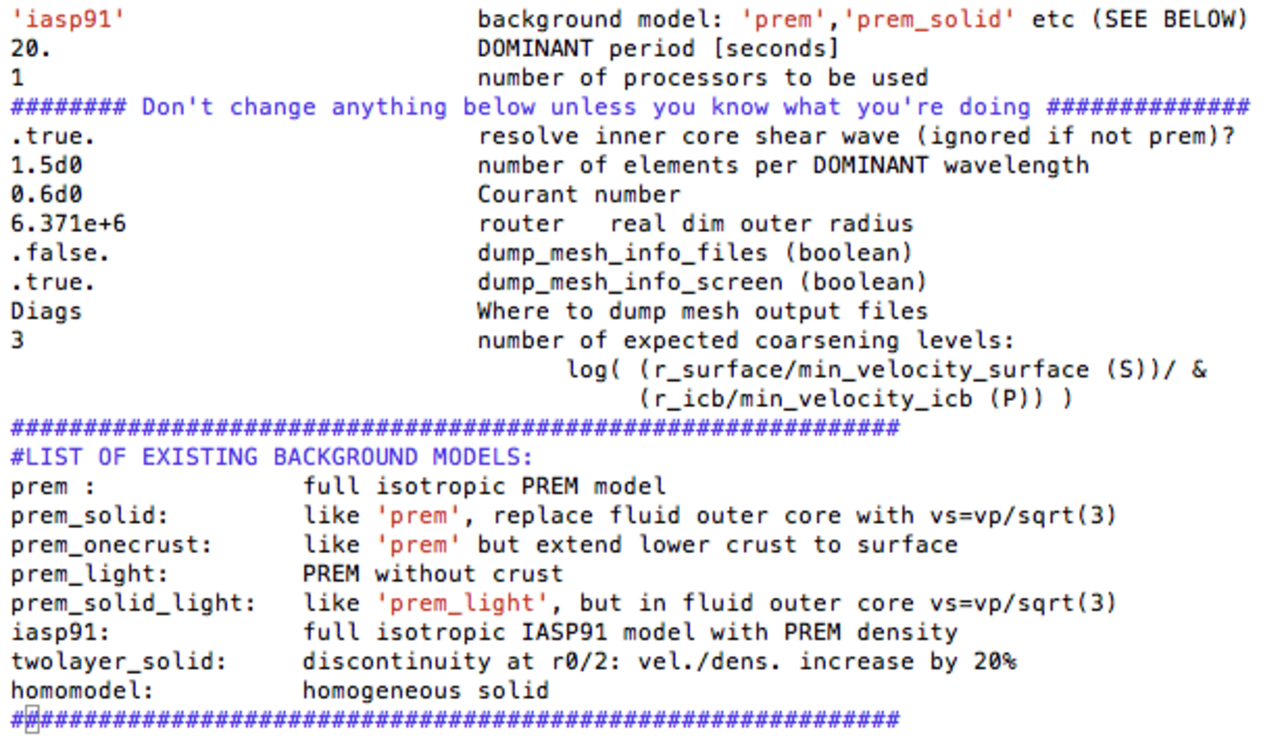
\includegraphics[scale=0.6]{inparam_mesh.eps}
% % \caption{\textit{{\tt inparam\_mesh}: defines all relevant parameters, mostly self-explanatory. }}
% % \end{center}
% \lstset{frame=single,basicstyle=\footnotesize, breaklines=true }
% \lstinputlisting{../MESHER/inparam_mesh.TEMPLATE}
% % \end{figure*}
% 
% \noindent \textit{Basic set of parameters} to be edited:
% % TODO: parameter names as in the input files
% % TODO: new switch: dump_vtk
% \begin{itemize}
%     \item \textbf{background models}: Be sure that the string defined here exists in 
%     {\tt background\_models.f90}. Adding new background models is explained further below.
%     
%     \item \textbf{dominant period:} This is the seismic source period at which
%     dominant parts of the spectrum are propagated. Note that this is different
%     from other codes in which the maximal frequency may be specified.  In most
%     applications, the solver should be run using a Dirac delta function and
%     then convolved a posteriori with the source-time function (STF).
% %     %In that
% %     case the pure simulation results contain high-frequency numerical noise
% %     beyond the mesh resolution, but the convolution eradicates those (even
% %     better than if a non-white spectrum STF is inserted as the source, since
% %     the spatial point source also introduces aliasing, which can only be taken
% %     care of via the above-mentioned posteriori convolution.
%     % TODO: sure? should this not be a linear effect? notes on stf seems a bit
%     % misplaced here, more relevant for SOLVER then MESHER
%     
%     \item \textbf{number of processors}: needs to be 1, 2, 6 or a multiple of
%     4. To get a suggestion for optimal decomposition, run the Mesher with \#proc
%     smaller or equal 4 and check the OUTPUT file. Then change the number in the
%     input file and rerun the mesher.
% 
%     \item \textbf{coarsening levels}: Keep this at 3 if applied to any typical earth models
%     (2 for 'light' models without crust), as this number reflects the overall
%     change in velocity between the surface and the deep interior.  if the total
%     global variation in wave speed is significantly different, other options
%     may be convenient here. This applies to other spheroidals, homogeneous or
%     simply layered models.
% \end{itemize}
% 
% \newpage
% \noindent \textit{Advanced set of parameters} to be edited:
% 
% \begin{itemize}
%     \item \textbf{resolve inner shear wave:} This should always be set to true.
%     If false, then the inner core is assumed fluid but the saved CPU cost is negligible.
%     
%     \item \textbf{polynomial order}: The polynomial order $N$ of the
%     Gauss-Lobatto-Legendre (GLL) basis within elements is often said to be
%     optimal at 4. However, this can be freely chosen, specifically if
%     convergence tests are needed, and Ref (5) suggests that higher polynomial
%     orders may be more cost-effective, depending on the constraints imposed by
%     the element mesh (e.g., thin crustal layers to be accomodated). The
%     ``optimal'' judgment stems from the fact that the minimal spacing of GLL
%     points depends on $1/N^2$, that is, the spectral convergence is
%     counteracted by a possibly quadratic decrease in the critical time step.
%     NB: 'Coarse grained' memory variables for efficient attenuation in the solver
%     are only implemented for polynomial order 4.
%     
%     \item \textbf{number of elements per wavelength}: This will be used to
%     compute the largest allowable grid spacing based on the dominant source
%     period and is intimately tied to the polynomial order $N$. See ref (5) for
%     a comprehensive analysis on how to choose the parameters if necessary.  If
%     the seismograms contain unreasonable noise (usually high-frequency tails),
%     are inaccurate or otherwise different than a reference solution or data,
%     try to increase this value. This will result in a denser mesh at higher
%     simulation cost (possibly more processors), but deliver more accurate
%     results. The absolute minimum number of grid points per maximum wavelength
%     for S waves is about 4.5 (i.e., this parameter times $N$). See ref (3) and
%     (5) for details.
%     
%     \item \textbf{Courant number}: Defines the stability criterion to choose
%     the critical time step.  0.6 is the heuristically determined maximal value
%     for any realistic applications. If the solver explodes, decrease this
%     number. Note that dispersion errors increase with propagation distances
%     (counted in wavelengths), and for large distances one should  choose a
%     smaller time step than the critical one (which is the one suggested by the
%     output of the mesher in {\tt mesh\_params.h}).
%     
%     \item \textbf{outer radius}: This is the same for IASP91 and PREM, but
%     should be changed accordingly if other models necessitate otherwise, or of
%     course if other spheroidals are considered. 
%     
%     \item \textbf{mesh info files}: These files become extravagantly large for
%     high-resolution meshes and are not needed by the solver, nor by any of the
%     current post-processing tools and as such should be kept .false. unless
%     significant changes or issues within the mesher are emerging.
%     
%     \item \textbf{mesh info screen}: This is extra output containing some more
%     details on the meshing process, but equally to the large files unnecessary
%     for any normal meshing procedure.
%     
%     \item \textbf{dump directory:} The directory where most of the output is
%     written. The posteriori {\tt movemesh} script moves all those files to the
%     permanent mesh location.
%     
% \end{itemize}
% 
% 
% \subsection{Running the mesher}
% Job submission is simple:\\
% {\tt ./submit.csh <optional queuing system>},\\
% where {\tt <optional queuing system>} can be {\tt lsf, torque, slurm,
% slurmlocal} at this point. Check {\tt ./submit.csh -h} for options.
% 
% \subsection{Changing the background model}
% This is traditionally the bottleneck of seismic code flexibility (in my very
% biased view)... so we've given considerable effort to making this task as
% primitive and decoupled from the rest of the code as possible. In principle,
% two options for new earth models exist: \\ (1) Parameterized, polynomial,
% piecewise continuous representation of wavespeeds $v(r)$,\\ (2) Discrete radial
% values of $v(r_i)$.\\
% 
% \noindent In principle, this should be entirely general such that you can dream
% up multiple fluid layers, discretely layered earths or other planets,
% ridiculous velocity variations, however we have not completed the fully fluid
% sphere just yet. As soon as your new model affects the overall change in
% velocity between surface and maximal value at depth, you will have to change
% the number of expected coarsening levels in {\tt inparam\_mesh} as indicated
% there. Also, the innermost layer needs to be thick enough to accommodate the
% inner cube of the mesh. \\
% 
% \noindent Two modules will need to be amended: {\tt model\_discontinuities.f90}
% and {\tt background\_models.f90}.  Note that {\tt background\_models.f90} is
% copied to the Solver by {\tt movemesh} such that additions will be
% automatically accounted for in the Solver. 
% 
% \subsection{Anisotropy}
% % TODO
% 
% \subsection{Attenuation}
% % TODO
% 
% \subsection{Computational aspects}
% The simulations should be done within seconds to minutes for meshes above 5
% seconds.  Note that doubling the resolution (half the period) results in a mesh
% that is 4 times larger and has about half the time step, i.e. the solver takes
% double the time at 4 times more processors. Increasing the number of processors
% while keeping resolution constant will slow the mesher insignificantly, but in
% most cases speed up the solver substantially, but not linearly (the more
% message passing, the slower).  This mesher is completely serial but constructs
% the parallel mesh database needed in the solver (in pdb.f90), easily down to
% periods of about 3 seconds on typical memory chips ($\sim$ 2GB), and down to 1
% second on larger shared memories (e.g. 16GB).
% % TODO: this is a repetition
% 
% \begin{table}[h]
% \begin{tabular}{ccc}
% period & max  \\
%  T[s]  & nproc & memory [GB] \\
% \hline
%  50.0 &    8  &  $< 1$  \\
%  25.0 &   12  &  $< 1$  \\
%  20.0 &   16  &  $< 1$  \\
%   9.0 &   32  &  $< 1$  \\
%   4.4 &   64  &  $< 1$  \\
%   2.2 &  128  &  $ 3.5 $ \\
%   1.1 &  256  &  $13.0 $ \\
% \end{tabular}
% \end{table}
% 
% \subsection{Code structure and components}
% Check {\tt main.f90} for the general code structure. Meshing of the spheroidal
% is confined to the module {\tt discont\_meshing.f90}. The inner cube contains a
% coordinate transformation (see Theory section), which is done in {\tt
% meshgen.f90}. The domain decomposition is accomodated by {\tt
% parallelization.f90}, and the parallel database generated in {\tt pdb.f90}. You
% may wish to avoid diving into these murky modules unless your curiosity exceeds
% that of an average coding geek, or you encounter an issue.\\
% 
% \noindent\textbf{Domain decomposition }\\
% In {\tt parallelization.f90} we have an exactly load-balanced colatitudinal
% cake-piece decomposition for the outer spherical part of the mesh. The central,
% rectangular part is trickier. We employ a method that is based on the
% following principles:
% 
% \begin{itemize}
%     \item exact load balancing 
%     \item maximally 2 neighboring domains, i.e. each domain touches the axis
%     \item at least two elements thickness
%     % TODO: isn't this three?
%     \item spherical cake-piece decomposition as 'boundary condition'
% \end{itemize}
% 
% % TODO: note on new decomposition method
% 
% %Upon this, we construct the decomposition by approximating polynomials $s(z)$
% %of varying degrees. For the time being, this is only implemented up to 
% %16 processors, but no hard limitation. See the Theory section in this manual for details.
% 
% \subsection{Output}
% \underline{Needed by solver} \\
% {\tt mesh\_params.h}\\
% {\tt meshdb.dat0000,...,meshdb.dat00$<$nproc-1$>$}\\
% %{\tt unrolled\_loops.f90}\\
% {\tt background\_models.f90}\\
% 
% \noindent\underline{NOT needed by solver }\\
% Everything else (mostly in directory {\tt Diags/}) including various global 
% arrays such as valence.\\
% 
% \noindent {\tt mesh\_params.h}: \\
% This is a header file that contains all the static array sizes for the solver
% such that it does not need to allocate (a lot of) memory dynamically.
% Specifically, it documents all revelant mesh input parameters commented at the
% top, and some output information such as time step at the bottom.  The
% inclusion of this header into the solver requires recompilation for each new
% mesh. This header includes mesh sizes and is identical for each processor due
% to the exact load balancing.  The last line is added by {\tt movemesh} and
% indicates the location of the mesh database. If you move the mesh, make sure to
% change this line accordingly!!  \\
% 
% \noindent {\tt meshdb.dat00*}: \\
% These are the complete databases for each processor of the solver simulations.
% They contain the skeleton mesh, regions, boundary information (axis, free
% surface, solid-fluid boundary, processor boundary), and basically everything
% needed for a full simulation except for the source-receiver specification which
% is an input for the solver. \\
% 
% \noindent After these two crucial output file types are written, the mesher
% reloads them as a simple test on some of their dependencies. More comprehensive
% tests are performed in the solver. \\
% 
% \noindent\textbf{\underline{Prepare files to be used in solver}}\\
% Use the script {\tt movemesh} to transfer all relevant files to the directory
% ../SOLVER/MESHES. 
% % TODO  I think this is ouddated. double check
% %Using this script is crucial since it adds a line to the {\tt mesh\_params.h}
% %header file to indicate the location of the large mesh databases.
% 
% \subsection{Mesher Post-processing/quality control }
% \begin{figure*}[htb]
%     \begin{center}\label{fig:mesh_vp}
%         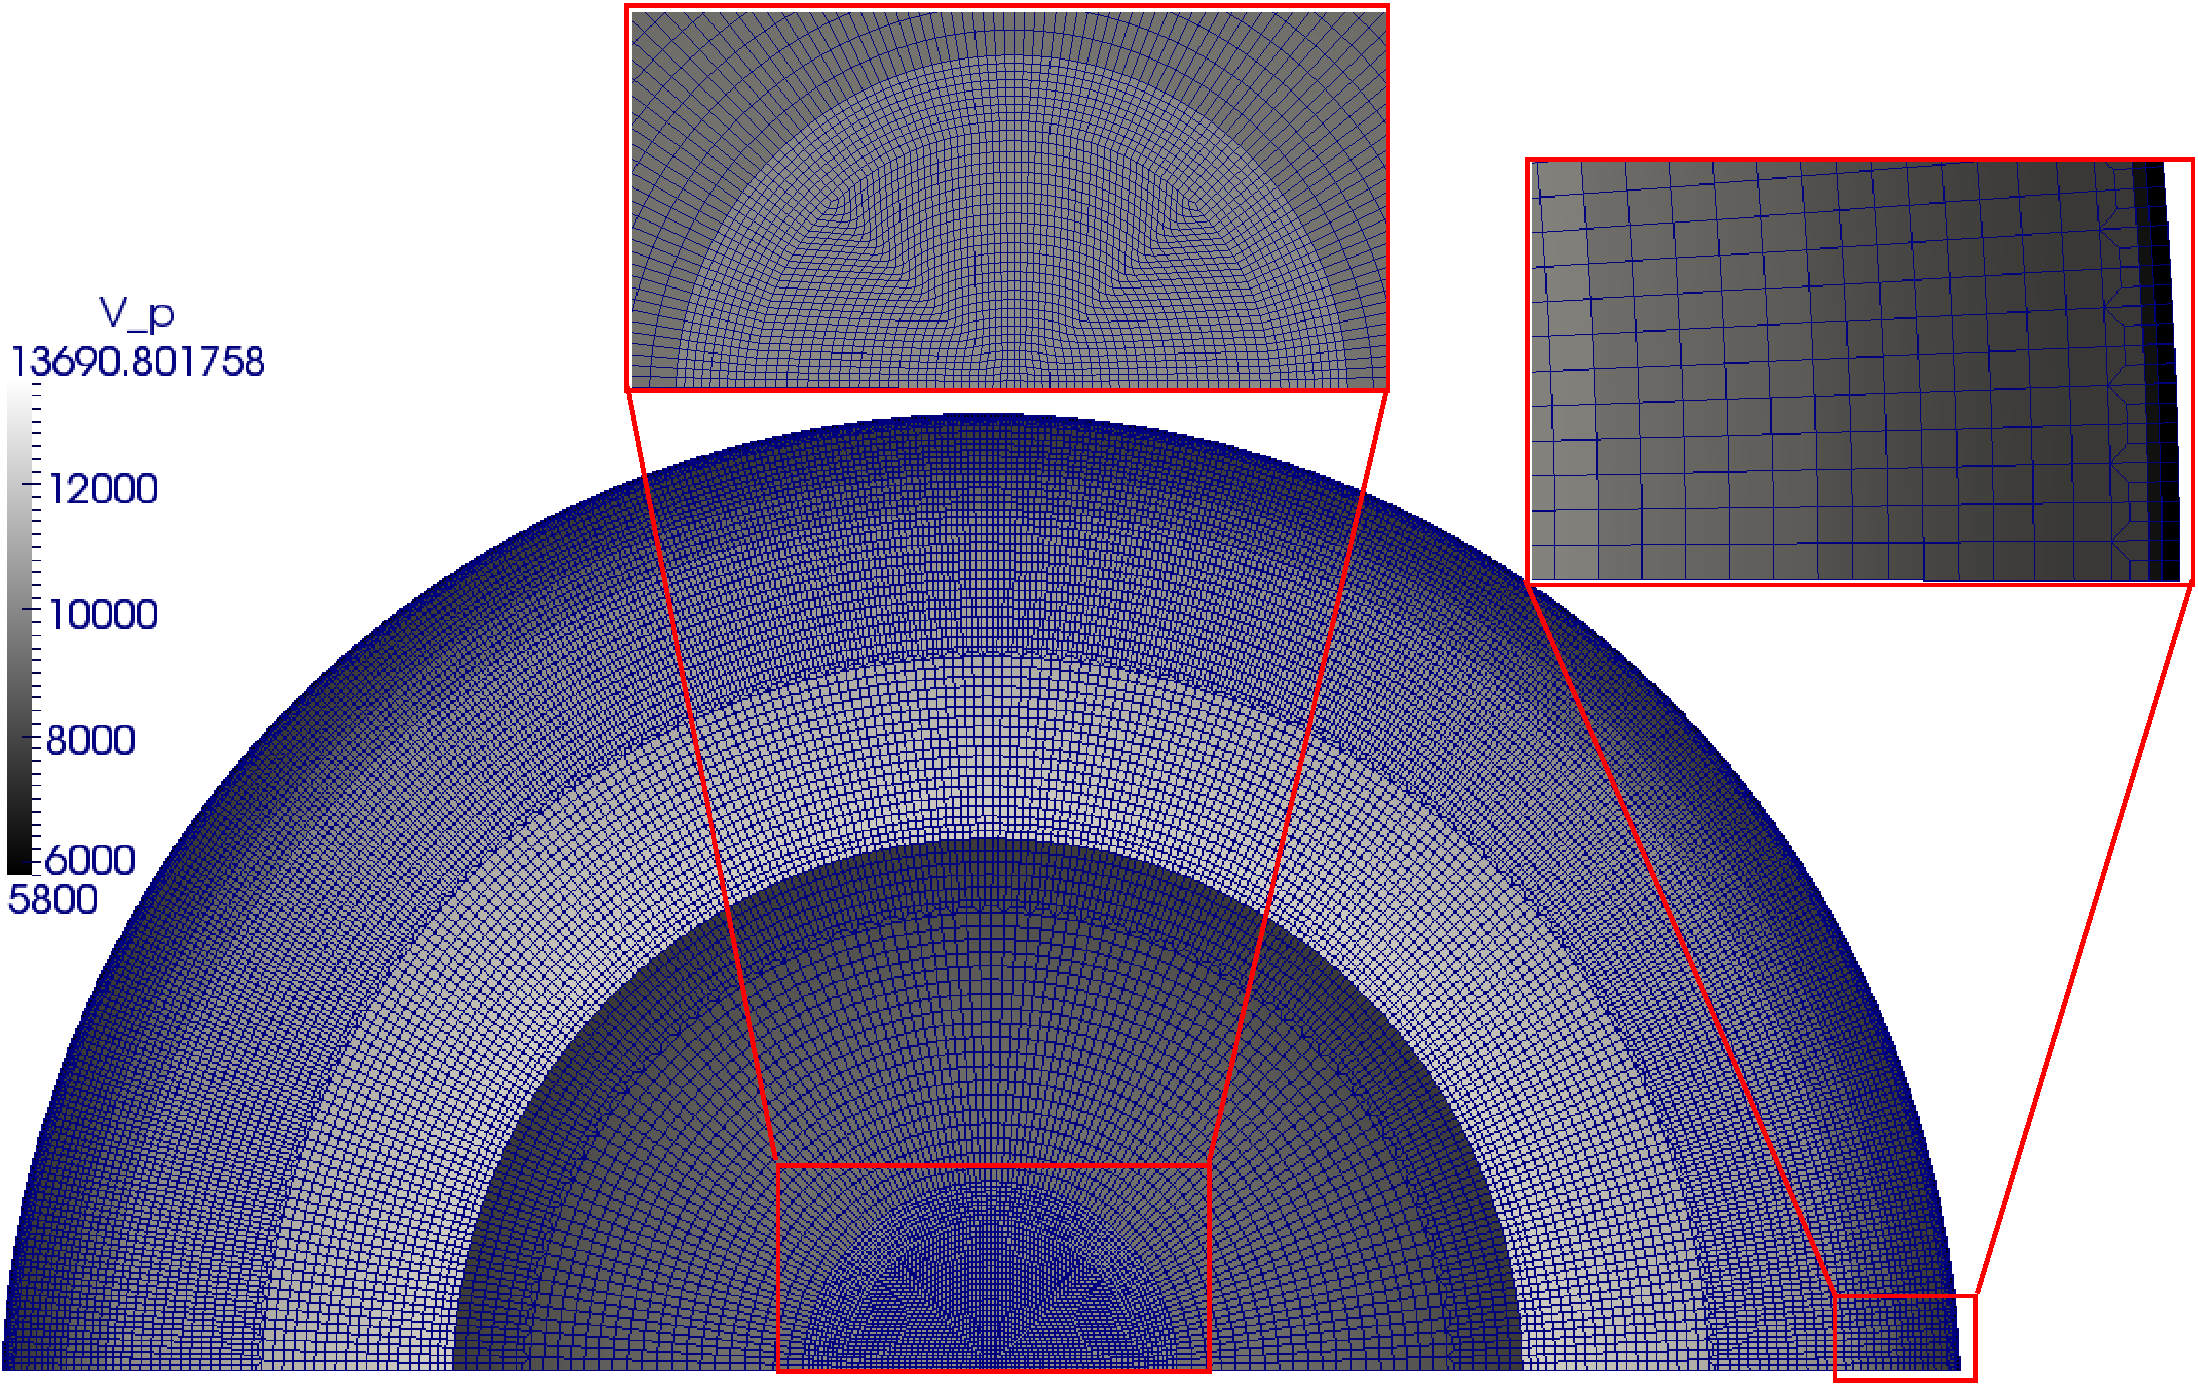
\includegraphics[scale=0.45]{mesh_vp_fig.pdf}
%         \caption{\textit{The elemental mesh (blue lines) for IASP91 at 20
%         seconds superimposed on the $v_p$ velocity.  The plot is derived
%         straight from the file {\tt mesh\_vp.vtk} produced by the mesher. Zoom
%         sections of the central region and crust/upper mantle are added to
%         highlight the topological features.}}
%     \end{center}
% \end{figure*}
% %
% \noindent Generic output includes various {\tt *.vtk} files on the elemental
% mesh with media properties (see Fig.~\ref{fig:mesh_vp}) as well as a host of
% other plots with respect to Courant number, points per wavelength, period, time
% step etc, and domain decomposition.  All of these files are moved to the
% permanent mesh location via {\tt movemesh} and can be easily viewed with {\tt
% paraview}. Turn on the \textit{surface with edges} and \textit{data} features
% to visualize the element mesh and medium properties, respectively.
% 
% \subsection{Cautions}
% Fully operational in single or double precision, so please \textbf{avoid using
% the -r8 (enforced double precision) flag}, since the output expects single
% precision for certain arrays (especially in vtk).
% %TODO do we ever use double precision?
% 
% \subsection{Issues}
% The hmin/hmax vtk output files have strangely large values, but the period and
% dt ones are fine.
% %TODO up to date?
% 
% \subsection{Mesher To Do}
% General cleanup, documentation, parallelization, netcdf database.
% %TODO fits in the general todo list at the very end of the manual
% 
% \newpage
% \section{Solver}
% Picks up the header from the mesher into its compilation to solve the
% elastodynamic 3-D equations of motion for spherically symmetric earth models in
% a 2-D computational domain using message-passing for the parallelization. The
% full seismic moment-tensor $M_{ij}$ is accounted for by four separate
% simulations: two monopole, one dipole, and one quadrupole simulation have to be
% done to sum up to the 6 independent elements of $M_{ij}$.  The software has the
% additional feature of computing and saving entire wavefields that form the
% basis of full-wave based, multiple-frequency sensitivity kernels. This output
% is included in the solver, but the calculation of kernels needs to be done
% elsewhere.  Detailed information on the various components of the code are
% included as comments to the respective modules and routines. Here, we give a
% simple overview over the main parts. 
% 
% \newpage
% % TODO: Wenn ich noch ein newpage sehe...
% % \subsection{Installation and compilation}
% % \begin{enumerate}
% %     \item If first used or new modules are added to the Solver code,
% %     use {\tt ./makemake.pl } to create a new Makefile.    
% %     %TODO Note on compilerflags for netcdf
% % 
% %     %\item Copy {\tt mesh\_params.h} from the desired mesh into the source code directory: 
% %     %It contains a last line that links to the location of the database such that 
% %     %these possibly very large files do not need to be copied. % actually they were copied to the rundir anyway
% %     % TODO note on new method: MESHNAME in inparam_basic
% % 
% %     \item Compile: {\tt make clean; make}
% %     \item Make sure that executable {\tt xsem} exists.
% % \end{enumerate}
% % TODO: Completely irrelevant by now.
% 
% %\subsection{Pre-processing}
% %The {\tt UTILS} directory contains some utilities that may be useful in 
% %choosing the right input parameters. 
% 
% \subsection{Input}
% 
% \textit{Automatically taken from mesher:} \\
% {\tt mesh\_params.h}: header including array sizes necessary for the compilation\\
% {\tt meshdb.dat00\*}: mesh databases for each processor\\
% %{\tt unrolled\_loops.f90}: unrolled loops and unit-stride cache access for given polynomial order\\
% % now generalized
% {\tt background\_models.f90}: all background models. Needs to be the same as in mesher\\
% % TODO copied over automatically
% 
% \noindent Any changes to Solver code, background model, mesh, polynomial order etc. require 
% recompilation. The above input files are fully automatic and need not be changed for all intents 
% and purposes of the Solver.\\
% 
% \noindent \textit{Input files for the Solver:} \\
% % TODO update!!!
% \noindent {\tt inparam, sourceparams.dat, receivers.dat}\\
% These 3 solver input files may be changed without recompilation of the solver 
% source code. We will describe these files at length in the following. PLEASE do not shy away from the 
% length of this section.... the input is fairly easy to understand and manipulate, 
% we simply intend to comment as much as possible on all options!\\
% 
% % TODO update!!!
% % \begin{figure*}[htb]
% % \begin{center}
% % \includegraphics[scale=0.6]{inparam.eps}
% \lstset{frame=single,basicstyle=\footnotesize, breaklines=true }
% \lstinputlisting{../SOLVER/inparam_basic.TEMPLATE}
% % \caption{\textit{{\tt inparam}: defines all relevant parameters, mostly self-explanatory. }}
% % \end{center}
% % \end{figure*}
% %
% \noindent {\tt inparam}:
% \begin{itemize}
% % TODO update!!!
%     \item \textbf{number of simulations}: Keep this at 1 for the time being,
%     this is not completed yet.  If you wish to simulate full moment tensors or
%     forces at once, do that via {\tt submit.csh}.
% 
%     \item \textbf{seismogram length:} Useful to check this via a ray tracer
%     (taup) before choosing, the overall CPU cost scales linearly with this
%     length.
% 
%     \item \textbf{time step}: If you keep this at 0.0, the code chooses the
%     critical time step as specified in {\tt mesh\_params.h}.  We suggest to
%     choose a lower value than this critical value, at best some  integer
%     multiplicative of the seismogram sampling specified further below. The CPU
%     cost scales inversely linear with the time step.
% 
%     % TODO symplec does NOT work atm
%     \item \textbf{time scheme}: see {\tt time\_evol\_wave.f90} for details.
%     {\tt newmark2} is the traditional 2nd-order scheme, {\tt symplec4} is a
%     PEFRL scheme of 4th order, about 2.5 more CPU time required than the
%     Newmark scheme but significantly more accurate. See ref(5) for a detailed
%     analysis and rules of thumb for choosing the optimal time scheme.
%     Generally, if the setup requires seismograms at more than 100 wavelengths
%     in distance, we suggest using the symplectic scheme. The memory
%     requirements for the symplectic scheme are in fact *lower* due to avoiding
%     the acceleration as a full wavefield. See the section on time schemes
%     further below on more information.
%     
%     \item \textbf{period}: Should keep this at 0.0 unless one wishes to test
%     accuracy for constant mesh at varying frequencies, or somehow the
%     simulations show inaccuracies. This choice is ignored if a delta function
%     is used as the source time function (in {\tt sourceparams.dat}), which
%     should be the preferred option unless wavefield snapshots (for propagation
%     movies etc) are needed. 
% 
%     \item \textbf{source file type}: Functional choices are {\tt separate} and
%     {\tt cmtsolut}.  {\tt separate} invokes the generic source file {\tt
%     sourceparams.dat}, and {\tt cmtsolut} the {\tt CMTSOLUTION} format. See
%     next section for details on these files. 
% 
%     \item \textbf{receiver file type}: Functional choices are {\tt colatlon}
%     and {\tt stations}.  {\tt colatlon} invokes the generic receiver file {\tt
%     receivers.dat}, and {\tt stations} the {\tt STATIONS} format. See two
%     sections down for details on these files. 
% 
%     \item \textbf{seismogram sampling rate}: Keeping this at 0.0 saves
%     seismograms at the time step sampling rate. Choosing values larger than the
%     time step may be useful to maintain a sampling rate equal to that of, e.g.,
%     data. Note though that keeping this value too high will result in crude
%     seismograms which loose valuable frequency information.
%     
%     \item \textbf{data and info output paths}: We suggest to keep those as
%     defined; {\tt Data} contains all the large output such as seismograms and
%     wavefields and all associated information. {\tt Info} contains additional
%     information files, e.g. on processor-specific output and properties. 
%     
%     \item \textbf{Save global snapshots}: Saves the displacement wavefield at
%     discrete time intervalls for posteriori compilation into a wave propagation
%     movie. These files are LARGE!  Only needed for visualization, understanding
%     certain wavefield features, but should be generally turned off. The
%     post-processing scripts turn these wavefields into a 3D global wave
%     propagation movie if saved. NOTE: if this is set to {\tt .true.}, then a
%     Dirac delta source doesn't make sense since the spurious high-frequency
%     signals cannot be filtered a posteriori. 
%     
%     \item \textbf{snapshot time interval}: Time in seconds between frames for
%     the above snapshots of the propagating global wavefield. Obviously the
%     output size depends directly on this intervall...  For decent movies we
%     suggest to keep this at 1-2 frames per seismic period.  
% 
%     \item \textbf{save wavefields for kernels}: So long as the kernel code is
%     not available, this is pretty useless since the resultant wavefields are
%     subjected to an extensive amount of operations (rotations, coordinate
%     transformations, frequency-domain transformations, convolutions, filtering)
%     to arrive at sensitivity kernels. Setting this to false ignores the rest of
%     the choices in this output section for sensitivity kernels. CAUTION: These
%     files are gigantic for high resolutions!
%     
%     \item \textbf{Samples per period}: Should be at least 2 to fulfill Nyquist,
%     but more are highly recommended for the purpose of picking time windows
%     when computing static kernels, e.g. 8-10.
%     
%     \item \textbf{source vicinity in wavefields}: Sensitivity kernels exhibit
%     large values right around the source and receiver. Apart from ignoring this
%     ({\tt igno}), we offer the possibility to simply {\tt mask} this region
%     with smaller values.  An analytical calculcation for homogeneous regions is
%     in the making.
%     
%     \item \textbf{starting/ending GLL point index}: Option to save only select
%     GLL points per element for the kernel wavefields. Choosing 1,1 means only
%     interior points, which maintains a smooth sampling (due to the GLL point
%     clustering near the element boundaries) and avoids the peculiar and tricky
%     issue of defining numerically accurate strains on discontinuities.
%     
%     \item  \textbf{energy}: avoid this unless you are specifically interested
%     in the kinetic, potential and total energy of the solid, fluid and global
%     domains since it involves a full evaluation of the stiffness matrix and is
%     therefore quite CPU (and memory) intensive. 
%     
%     \item  \textbf{homogeneous parameters}: This is mainly for testing purposes
%     and should be turned to false otherwise. Only possible for purely solid
%     models and only really useful for testing/debugging.
%     
%     \item \textbf{homogeneous P-vel etc}: Populates the entire domain with this 
%     homogeneous media characterization if exclusively solid.
%     
%     \item \textbf{analytical solution around source}: An analytical reference
%     solution to test the accuracy of near-source radiation in a homogeneous
%     model. Should only be on if this is relevant.
%     
%     \item \textbf{add heterogeneity}: Turning this {\tt .true.} invokes an
%     additional input file called {\tt inparam\_hetero}.  This perturbs the
%     background model in a specified region (defined by elements within a range
%     of specified coordinates) by percentile changes to velocities $v_p$, $v_s$,
%     and density $\rho$. This part of the code is still under development but
%     contains a number of different types of heterogeneties, all of which are
%     defined in {\tt lateral\_heterogeneties.f90}. See more details in the
%     separate section below.  This should generally be set to false unless you
%     specifically wish to analyse waveform effects due to such 2.5-dimensional
%     heterogeneties. 
%     
%     \item Setting the next two lines to false (do mesh tests, save large test
%     files) avoids extensive checks on the mesh, model, discontinuities etc.
%     Upon a new mesh, this may be turned to true at least once (same after any
%     source code changes), otherwise it's fine to avoid these tests and large
%     files.
%     
%     % TODO note on compiler flag
%     \item A new (Nov. 2011) feature is the I/O using the netcdf standard. This
%     is extremely beneficial for platform-independent binaries, direct access,
%     reducing the number of written files, and is installed on every
%     well-managed computer cluster. However, installing these libraries can be
%     tedious. For this case, we have left the option to go with fortran binary.
%     The decision is two-fold; the first one already taken in {\tt makemake.csh}
%     since the makefile needs to know whether the libraries are installed. Even
%     if installed, one can still turn the netcdf option off by putting binary
%     here. 
% \end{itemize}
% 
% \noindent \textbf{Source specification.}\\
% Includes all parameters describing the earthquake (or other) source, which are:
% radiation patterns and magnitude, source location (depth, latitude, longitude),
% source-time function.  As of now, the code only computes point sources (finite
% faults are in development), and simply takes the closest grid point as the
% location. Mislocation errors are given in OUTPUT\_$<$dir$>$.\\
% 
% % TODO Note on sourceparams only with single mode
% \noindent {\tt sourceparams.dat}
% % \begin{figure*}[htb]
% %     \begin{center}
% \lstset{frame=single,basicstyle=\footnotesize, breaklines=true }
% \lstinputlisting{../SOLVER/inparam_source.TEMPLATE}
% %         \caption{\textit{{\tt sourceparams.dat}: Specifies source properties using its own format.}}
% %     \end{center}
% % \end{figure*}
% 
% \begin{itemize}
%     \item  \textbf{magnitude}: The code runs in SI units, and the moment tensor
%     is given in [N m], i.e. $10^{20}$ here for moments equal $10^{27}$ dyn cm
%     in the {\tt CMTSOLUTION} format further below. The moment-tensor elements
%     here are given in global cartesian coordinates (Greenwich), such that they
%     are subjected to rotations if the source is not along the axis.
% 
%     \item \textbf{excitation type}: earthquakes only contain mono-, di-,
%     quadrupole radiation
% 
%     \item \textbf{radiation pattern}: \\
%     monopole: {\tt explosion, mzz, mxx\_p\_myy, vertforce}\\
%     dipole: {\tt mxz,myz, yforce, xforce} \\
%     quadrupole: {\tt mxy, mxx\_m\_myy}\\
%     This is overdetermination, granted, but still a sensible check on whether 
%     one has the anticipated source defined - a VERY COMMON *source* of swiftly 
%     running wrong simulations! Consistency checks are included at run time.
% 
%     \item \textbf{source depth}: NOTE: DEPTH in KM, NOT radius!
% 
%     \item \textbf{source colatitude and longitude}: If the source is located
%     away from the axis, the code rotates the entire source-receiver geometry
%     such that the simulation runs with a corresponding source at the axis. This
%     should be invisible to the user, but means that the raw seismogram output
%     is not at the correct azimuth: This is accomodated in the post processing
%     stage (see below). 
% 
%     \item  \textbf{source time function}: Dirac Delta (single forces)/Heaviside
%     (moment tensor) should be used in all cases except for wavefield snapshots
%     or specific tests.  This instantaneous source detonates at the first time
%     step of the seismogram sampling ({\tt t(seis\_it)}). Details below.
% \end{itemize}
% 
% \noindent {\tt CMTSOLUTION}\\
% % \begin{figure*}[htb]
% %     \begin{center}
% \lstset{frame=single,basicstyle=\footnotesize, breaklines=true }
% \lstinputlisting{../SOLVER/CMTSOLUTION.TEMPLATE}
% %         \caption{\textit{{\tt CMTSOLUTION}: Specifies source properties using the Harvard CMT format. Note that the source-time function
% %         is added as the first string in the first line, if none is added, then a Dirac delta distribution is assumed.}}
% %     \end{center}
% % \end{figure*}
% 
% \noindent If {\tt CMTSOLUTION} is specified, the moment tensor elements adhere
% to the spherical system (or what is called the ``local'' {\tt (x,y,z)}), i.e.
% is invariant to rotations.  If the source is not at the pole, then the receiver
% coordinate system is automatically set to spherical, irrespective of {\tt
% inparam}: this is so since in the cylindrical case, the rotated receiver system
% would need additional rotations, whereas the spherical system does not. The
% source time function in CMTSOLUTION can be specified by adding it as a string
% to the first line. If not specified, the default is the Dirac Delta
% distribution. Half duration corresponds to what we take as the dominant period
% in seconds, and time shift is ignored for now.  Depth is in kilometers,
% latitude and longitude in degrees, and the moment tensor elements in [dyn cm],
% i.e. $10^7$ larger than the corresponding entries in {\tt sourceparams.dat}! \\
% 
% \noindent \textbf{Source-time function.}\\
% %
% \noindent Choices are between impulsive sources (Dirac Delta distribution,
% Heaviside, see below) and smooth sources with a limited frequency band
% (Gaussian, Ricker, derivative of Ricker and a wiggly wavelet with boxcar
% frequency spectrum (called {\tt heavis})), see the Figure for their shapes.
% The distributions start rupture at $t=t({\rm seis\_it})$ (the first time step
% counted in the seismogram sampling); the Gauss, Ricker and derivatives have the
% wavelets centered at $t=1.5 \,T_0$, and the {\tt heavis} function is shifted by
% $300 s$ due to its very long wavelength components. These time shifts are
% recorded and saved into post processing, but it is crucial that users are aware
% of these shifts when comparing to data or other methods. \\
% 
% % \begin{figure*}[htb]
% %     \begin{center}
% %         \includegraphics[scale=0.45]{stfs.eps}
% %         \caption{\textit{The smooth source time functions for a period of
% %             $T_0=20$s. Note the shifted center for each function ($1.5 T_0$ for
% %             all except the wiggly wavelet which is shifted by $300s$). The
% %             amplitude includes the scalar moment of the source. }}
% %     \end{center}
% % \end{figure*}
% % 
% % \begin{figure*}[htb]
% %     \begin{center}
% %         \includegraphics[scale=0.45]{power_spectrum_stf.eps}
% %         \caption{\textit{Power spectra of the source time functions from the
% %             previous Figure.}}
% %     \end{center}
% % \end{figure*}
% 
% \noindent \textbf{Discrete Dirac distributions.}\\
% Hidden in the code are several crucial decisions upon how to approximate Dirac
% and Heaviside distributions with discrete and possibly heavily downsampled time
% series. These aspects are dealt with in subroutine {\tt
% compute\_numerical\_parameters} in module {\tt parameters.f90}, and subroutine
% {\tt delta\_src} in {\tt module sources.f90}.  In summary, a triangular Dirac
% is taken if there is no downsampling, leading to perfect reconstruction of the
% Dirac properties. If seismograms or wavefields are downsampled (as specified in
% {\tt inparam}), then one needs to revert to "smooth" functions that replicate
% Dirac properties. Amongst a choice of functions, we set the default to a tight
% Gaussian scaled to honor the Dirac integral unity, whose half width depends on
% the time step of the SEM, the seismogram/wavefield sampling rate, and
% mesh-based period. In principle, we observe acceptable reconstruction of
% Green's functions if more than 10 points per (mesh) period are used. The
% discrete Dirac functions are shifted such that they (1) start at zero smoothly,
% (2) are exactly sampled by all the sampling rates (SEM time step, seismogram,
% wavefield sampling rates). The crucial parameters for these shifts are saved
% for the post processing step and dealt with there. In principle, users should
% not need to worry about these issues, but be aware of the sensitivity of
% results upon these specifications. Heaviside approximations are simply
% numerically integrated from the Dirac distributions.\\
% 
% \textbf{WARNING:} The implementation of approximate/smooth Dirac distributions
% has not yet been implemented for the symplectic schemes, as these require
% different temporal sampling and hence more layers of if's, dont's, and special
% cases in the definition of these approximate Diracs.
% 
% \noindent \textbf{Receiver specification.}\\
% At this point two receiver file formats are accepted, both of which specify the
% (co-)latitude and longitude of the receivers. The code simply finds the closest
% grid point which, due to the crustal discretizaton, is usually of negligible
% difference. Check {\tt OUTPUT\_$<$dir$>$} to see how mislocated they are.  Note
% that specifying a non-zero longitude is essentially just saved to output and
% loaded in the post-processing stage. This is due to the 2D nature of the
% computational domain, and the 3D location is analytically reconstructed a
% posteriori. Also note that these are \textit{globally fixed coordinates}: If
% the source is not meant to be beneath the North pole (as specified in the
% source input file), then the combined source-receiver geometry is rotated
% within the code such that the source coincides with the North pole as necessary
% for the simulation.  To retrieve the response at the proper location on the 2D
% surface, this involves component rotations and is taken care of in the post
% processing stage. In the current workflow, is intended that the user can safely
% ignore these cumbersome operations so long as one appropriately applies the
% post processing operations. \\
% 
% \noindent {\tt receivers.dat}\\
% If {\tt colatlon} is specified in {\tt inparam} (see above), then a file called
% {\tt receivers.dat} in the source-code directory is needed. This file contains
% a simple list of co-latitudes and longitudes.  The first line denotes the
% number of receivers to follow, i.e. length of file minus one:\\ 
% {\tt <number of receivers>\\
% <rec. 1 colatitude [deg]> <rec 1 longitude [deg]>\\
% <rec. 2 colatitude [deg]> <rec 2 longitude [deg]>}\\
% 
% \noindent 
% A script called {\tt create\_receiver\_file.bash} is provided in the {\tt
% UTILS} directory to generate such files with constant spacing. Choose number of
% receivers as an argument and the resultant file will spread receivers along the
% colatitude between 0 and 180 degrees.\\
% 
% \noindent {\tt STATIONS}\\
% This choice requires a file called {\tt STATIONS} in the source-code directory.
% As an example, in the {\tt UTILS} directory you will find a file named {\tt
% STATIONS\_all\_15aug2008\_cleaned} with more than 3000 actual seismometer
% locations.  The file structure is generic, but do note that this format uses
% the latitude rather than colatitude (in opposite to the {\tt receivers.dat}
% format).  Elevation and burial are ignored for the time being. Station names
% are transfered to the output seismograms in {\tt Data}, see section on output
% for more details.
% 
% \subsection{Adding lateral heterogeneities}
% % \begin{figure*}[htb]
% %     \begin{center}
% \lstset{frame=single,basicstyle=\footnotesize, breaklines=true }
% \lstinputlisting{../SOLVER/inparam_hetero.TEMPLATE}
% %                 \includegraphics[scale=0.5]{inparam_hetero.eps}
% %         \caption{\textit{{\tt inparam\_hetero}: defines the region of lateral
% %             heterogeneities and medium variations.}}
% %     \end{center}
% % \end{figure*}
% % \noindent 
% 
% \textbf{NOTE:} This section has been heavily expanded and used most recently
% (fall 2011), but not yet tested in full extent. Everything concerning lateral
% heterogenities is confined to module {\tt lateral\_heterogeneities}.\\
% 
% If the boolean {\tt add\_heterogeneities} in {\tt inparam} is set to true, then
% a file named {\tt inparam\_hetero.dat} is required which specifies (1) a region
% within which heterogeneities are added and (2) the perturbations of the model
% parameters in percent with respect to the background model. The example in the
% Figure describes a boxcar atop the core-mantle boundary in which variations are
% constant, resembling simplistic models of an Ultra-Low Velocity Zone. The
% heterogeneity is added to the background model in the module {\tt
% get\_model.f90}, routine {\tt read\_model.f90}. The simple case described here
% is no inherent limitation but simply the first step into the direction of
% adding heterogeneities. More complex shapes can be defined as well as
% non-constant model perturbations, but this involves modifying the input file
% and the routine in which this takes place. \\
% 
% \noindent \textbf{IMPORTANT NOTE}: AXISEM is based upon the assumption of
% axially symmetric background models to rely on the specific radiation
% patterns that allow for a dimensional collapse to a 2D computational domain. If
% one adds lateral heterogeneities as above, the code simulates wavefields as if
% they penetrate a ring-like, tube structure that is invariant along the azimuth.
% This is often called 2.5-dimensional modeling. Thus, if one is only interested
% in the relative waveform impact of heterogeneous structures along the
% source-receiver plane, and in addition simulates at sufficiently high
% frequencies, then only a fraction of the ring structure will be ``seen'' by the
% transient wave. Although this has been common practice for many studies with
% various other codes beforehand, it is important to keep these topics in mind
% when interpreting results from lateral heterogeneities. Note also that while
% the structure is 1D (spherically symmetric) and, if the above is applied,
% locally 2.5D, the resultant wavefield is always the full 3D response to these
% background models.
% 
% % TODO note on discontinuities in the perturbations
% 
% \subsection{Running the solver}
% We use the following script to submit a parallel job from the source-code directory:\\
% {\tt ./submit.csh <run\_directory> <additional arguments>}\\
% 
% \noindent {\tt submit.csh}\\ 
% Check{\tt ./submit.csh -h} for argument options.  This script performs a number
% of crucial operations for the code to run, e.g. adheres to the source and
% receiver specifications, creates subdirectories, copies relevant files into
% them, and can submit a full moment (4 simulations) simultaneously.  The {\tt
% <run\_directory>} can be a global or local path. In most cases, one should keep
% the source code in a safe (backed up) location, whereas {\tt <run\_directory>}
% may be a faster/larger scratch system.  By experience, it is good practice to
% include all crucial parameters into the name of the run, specifically: mesh
% resolution, background model, number of processors, moment tensor type, source
% depth, source time function, and output choices (e.g. wavefield snapshots,
% kernel wavefields), e.g.  {\tt PREM\_20s\_NP2\_Mzz\_100km\_GAUSS0\_SNAPS}.  The
% script generates {\tt param\_sum\_seis} in the run directory containing the
% number of these simulations and their respective locations. 
% 
% \subsection{Computational aspects}
% \noindent A monopole simulation for a dominant period of 10 seconds on 2
% processors and one-hour long seismograms (without saving large wavefields)
% should take no longer than an hour, i.e. \textbf{real-time on a laptop} (see
% Table 1).  It is important to recognize that a simulation at half the dominant
% period compared to a previous simulation takes about 8 times longer if
% seismogram length is fixed: The mesh is about 4 times larger, and the time step
% about twice as small.  Note that monople source types run faster and require
% less RAM than dipoles and quadrupoles.\\
% 
% % TODO replace with new figures
% \begin{table*}[htb] 
%     \begin{minipage}{150mm}
%         \caption{ \textit{RAM and CPU requirements for simulations at dominant period 10s, PREM}.}
%         \label{apptable:matrix_op}
%         \vspace*{.2cm}
%         \begin{tabular}{@{}cccc}
%             nproc & RAM/CPU [MB] & seismogram length [s]& CPU time [s]\\
%             \hline\\
%             1 & 380 & 1000 & 1717\\
%             2 & 210 & 1000 & 1076
%         \end{tabular}
%     \end{minipage}
% \end{table*}
% 
% \noindent \textbf{Performance.} Our experience favors the Intel compiler using
% optimization flags {\tt -O3 -xHOST}, but Pathscale (not that they offer the
% compiler open-source now) performs very well too.  Performance can be severely
% hampered by writing to a different/slow file system, running a parallel job on
% nodes that are partly busy with other tasks, reaching the RAM limits (or
% swapping). In terms of input choices, saving wavefields for snapshots or
% sensitivity kernels take up significant portions of the CPU time as well. The
% Theory section contains some more details on performance checks.\\
% % TODO some trivialities, theory section removed
% 
% % new scaling tests
% \noindent \textbf{Scaling.} The code scales very well: both weak and strong
% scaling have shown above 90\%.  This is due to the exact load balance and
% minimal number of processor neighbors (two) as well as the asynchronous message
% passing. The Solver output contains some run-time information at the end, in
% which the time spent in crucial routines (assembly, time loop, saving
% wavefields) is calculated. 
% 
% \subsection{Code structure}
% \noindent {\tt main.f90} is the wrapper routine, and most of the relevant
% seismologically relevant routines are called from {\tt time\_evol\_wave.f90}.
% The overall code contains $\sim$ 200 potentially job-terminating if-statements
% which test a variety of generic issues prior to the time loop, and as such it
% should be fairly robust once the time loop is entered. \\
% 
% \noindent \textbf{Time loop.} 
% Several time schemes are included, most importantly the 2nd-order Newmark
% scheme and a symplectic 4th-order scheme. See next section for details.  Most
% of the heavy floating-point-operation-intensive number crunching happens in
% unrolled\_loops.f90, which is a routine optimized for faster cache access
% following Deville et al. 2003. 
% 
% \subsection{Choice of appropriate time schemes}
% In most other spectral-element codes, the 2nd-order Newmark scheme is the main
% option for time schemes. It performs fairly well for a certain parameter
% regime, so long as the time step is chosen with care. To obtain small
% dispersion errors for large propagation distances (e.g. over more than 100
% wavelengths), higher order symplectic schemes are more effective. See the
% Theory section or Ref (5) for more details.\\
% 
% \noindent \textbf{Newmark scheme.}
% The conventional explicit, acceleration-driven Newmark scheme of 2nd order.
% (e.g. Chaljub \& Valette, 2004). The mass matrix is diagonal; we only store its
% pre-assembled inverse at the stage of the time loop.  Explicit axial masking
% follows ref (2).  Note that the ordering (starting inside the fluid) is crucial
% such that no iterations for the boundary terms are necessary.  Also note that
% our definition of the fluid potential is different from Chaljub \& Valette and
% the code SPECFEM by an inverse density factor. This is the correct choice for
% our case of non-gravitating Earth models, but shall be altered once gravity is
% taken into account.\\
% 
% \noindent \textbf{Symplectic schemes.}
% Several higher-order time schemes are included that solve the coupled
% solid-fluid system of temporal ODE's using symplectic time integration schemes
% of 4th or 6th order.  The time step can be chosen 1.5 times larger than in
% Newmark, resulting in CPU times about 2.5 times longer than Newmark, but
% considerably more accurate. Consult Ampuero \& Nissen-Meyer (2011) for examples
% of when this choice should be more appropriate. Generally, for long propagation
% distances (say, $>$ 100 wavelengths), it is worthwhile considering this scheme.
% Note also that symplectic schemes actually occupy \textit{less memory} at run
% time.\\
% 
% \textbf{WARNING:} The implementation of approximate/smooth Dirac distributions
% has not yet been implemented for the symplectic schemes, as these require
% different temporal sampling and hence more layers of if's, dont's, and special
% cases in the definition of these approximate Diracs.
% 
% \subsection{At run-time} 
% Everything related to a run is located in the run directory: {\tt cd
% <run\_directory>; ls}\\ \noindent You should see an executable, input and
% header files, a file called {\tt OUTPUT\_$<$run\_directory$>$} (the file name
% may replace slashes with underscores if global paths are used) and files {\tt
% output\_proc00*.dat}, as well as time stamps eventually (the pre-timeloop CPU
% time may take a few minutes). Time stamps are written every estimated 1\% of
% the total runtime.  Min/max displacement values are recorded and may be a good
% starting point in deciphering a potential blow-up of the simulation. Note that
% this happens if the time step is too large, whereas inaccurate seismograms
% (containing high-frequency wiggles) happens if the grid spacing is too large.
% 
% \subsection{Output}
% The Solver produces vast amounts of various types of output, both in the {\tt
% Info} and {\tt Data} directories (as specified in {\tt inparam}. We will only
% cover the most relevant ones here, most other output is self-explanatory or
% well commented in the code, or irrelevant ;-) General information on the run
% can be found in {\tt simulation.info}, besides the generic standard {\tt
% OUTPUT\_<run\_directory>} and the processor-specific files {\tt
% output\_proc00*.dat}. Google-earth kml files that describe the input
% source-receiver geometry and, if necessary, the rotated one used in the code
% are provided in {\tt Info/src\_rec*.kml}.  The source-time function is in {\tt
% Data/stf.dat}. All of the following output is located in {\tt Data}.\\
% 
% \noindent \textbf{Seismograms}: \\
% Default output are seismograms at the epicenter, hypocenter, equator, and
% antipode. These are organized as (time, displacement component), and called
% e.g. {\tt seisepicenter1.dat} for the first component.  All other seismograms
% based on the chosen input ({\tt receivers.dat} or {\tt STATIONS}) contain the
% displacement components only (no time column). Seismograms from {\tt
% receivers.dat} are called {\tt recfile\_00*\_disp.dat} and {\tt
% recfile\_00*\_velo.dat} for displacement and velocity, respectively.
% Seismograms from {\tt STATIONS} contain the station name. Note that these
% seismograms are the collapsed-dimension equivalent, so in principle we advise
% to not touch them but rather proceed with post processing to properly rotate
% them to the correct location before any further analysis.\\
% 
% % TODO XDFM files
% \noindent \textbf{Wavefield snapshots}:\\
% Displacement snapshots are saved into files {\tt snap\_<proc number>\_<time sample>.dat}
% and saved across the entire mesh, additionally a corresponding mesh file is written.
% These wavefields are loaded into the post processing procedure and converted to 3D 
% movies.\\
% % 
% % % TODO is that to be used by anyone soon?
% % \noindent \textbf{Kernel wavefields and seismograms}: \\
% % Similar to snapshots, but the strain tensor needs to be computed on the fly
% % first, see {\tt time\_evol\_wave.f90}.  At this point, we offer two end-member
% % versions of dumping the fields to eventually calculate waveform kernels:
% % 
% % \begin{enumerate}
% %     \item \textit{displ\_only} dumps a minimal amount and requires extensive
% %     post-processing when calculating the kernels, but optimizes the SEM simulation
% %     in terms of memory, storage amount and CPU time.  Note that this method IS ONLY
% %     POSSIBLE IF ENTIRE SEM MESH IS DUMPED.  This means minimal permanent storage,
% %     minimal run-time memory, minimal CPU time, but extensive post-processing (need
% %     to compute strain tensor).
% %     
% %     \item \textit{fullfields} computes the entire strain tensor and velocity 
% %     field on-the-fly, resulting in more output (9 rather than 6 fields), 
% %     more memory and CPU time during the SEM, but no post-processing necessary. 
% %     This means maximal permanent storage, maximal run-time memory, maximal CPU time, 
% %     but no post-processeing necessary as these are the fields that 
% %     constitute density and elastic kernels.
% %     Any kind of spatial distribution can be dumped, meaning in the long run 
% %     this should be the more effective choice, and we recommend using this option.
% % \end{enumerate}
% 
% \noindent \textbf{Energy}: \\
% Time series for total, kinetic, and potential energy of global, solid and fluid
% domains.
% 
% \subsection{Cautions}
% The code should NOT be compiled with the {\tt -r8} flag (automatic double
% precision), since the vtk output assumes single precision. All sensitive
% parameters (e.g. coordinates) are kept at double precision when needed
% internally anyway...
% 
% \subsection{Issues}
% For 1.5 elements per wavelength (specified in {\tt inparam\_mesh}), there are
% still some spurious wiggles most notably at zero epicentral distance (the
% axis). Might come from the fact that meshing is not appropriately accomodating
% the Gauss-Lobatto-Jacobi basis near the axis, check {\tt discont\_meshing.f90}
% in the mesher.  Choosing a higher period or denser mesh takes care of this for
% the time being.
% 
% \subsection{Solver To Do}
% \noindent Physics: oceans, fully fluid sphere, (gravity, rotation)\\
% 
% % \noindent Kernel output: incorporate boundary kernels, wavelet compression or similar, writing wavefield snapshots into
% % frequency domain\\
% % TODO what about wrting the kerner in the first place?
% 
% \noindent Multiple source flexibility: Option to run 4 simulations for a
% complete moment tensor consecutively without changing input parameters, in
% combination with actual receiver and source coordinates (coordinate and
% component rotations) for seismograms and snapshot wavefield.  Also, the option
% to submit one parallel job distributed across 4*nproc processors to do the
% entire moment tensor and sum on-the-fly. Finally, the option to run multiple
% source depths in one parallel job submission: This has the advantage that only
% the dynamic wavefields and source term differ from one source to the other,
% i.e. one saves a lot of total memory compared to separate runs. Vision: One job
% submission (hundreds of processors) for the entire database...\\
% 
% % \noindent Embedded multiple simulations: Parts have been started (see the loop in {\tt main.f90}), but this is far from finished. 
% %   Two options should be done: \\
% %         1) Sequential 4 simulations for the full moment tensor, but invoked from within the code, not in the submit script\\
% %         2) Parallel runs for all 4 simulations, where all systems (mono/di/quadrupole are loaded simultaneously). Disadvantage that 
% %             monopole runs are faster... so any internal seismogram summation
% %             will lead to idle processes (unless completely parallelized such
% %             that each processor owns parts of each radiation type). This is a
% %             bit of recoding...\\
% % 
% %  -netcdf input (mesh database)\\
% 
% 
% \newpage
% \section{Post processing}
% Once the simulation is done, you'll have to run post processing in the run
% directory. This code performs the following crucial tasks:
% 
% \begin{itemize}
%     \item Load seismograms
%     \item Convolve seismograms with newly defined source time function and
%     seismic period
% 
%     \item Compute seismogram at correct azimuth
%     \item Sum individual seismograms to full moment tensor (if applicable)
%     \item Rotate seismogram components to new coordinate system
%     \item If available, plots seismograms using {\tt gnuplot} in pdf and gif
%     formats
% 
%     \item shifts seimograms such that the source-time function coincides with
%     time zero (either starting at negative time or at zero)
% 
%     \item Constructs a google-earth kml file that plots source-receiver
%     geometry on 3D surface, source information, and seismograms as images
% 
%     \item If applicable, loads wavefield snapshots and computes 3D wave
%     propagation for wavefields upon full moment tensor source, using the cubed
%     sphere on 2 surface (top and bottom) and two cross-sections (``cakepiece'')
%     inside the 3D sphere
% 
%     \item If available, computes theoretical traveltimes for the
%     source-receiver configuration using TauP
% 
%     \item Offers matlab script to plot record sections of all seismograms
% \end{itemize}
% 
% \noindent Before running this script, it is useful to check the parameter files
% for post processing that were automatically generated by the Solver based on
% assumptions about what you might be interested in:\\
% 
% % TODO new param_postprocessing file
% \lstset{frame=single,basicstyle=\footnotesize, breaklines=true }
% \lstinputlisting{../SOLVER/UTILS/param_post_processing}
% 
% \noindent {\tt param\_post\_processing}\\
% This file is automatically generated by the Solver but should always be checked
% before running the post processing.  If a full moment is submitted, then {\tt
% param\_post\_processing} is in the actual run subdirectory (usually called {\tt
% MZZ} etc).  {\tt post\_processing.csh} takes care of copying this into the main
% directory, but if you wish to edit it before processing, then copy one of them
% beforehand (e.g. {\tt cp MZZ/param\_post\_processing .}) and edit locally.\\
% 
% 
% \noindent \textbf{Run post processing}\\
% Inside the main run directory: {\tt ./post\_processing.csh}.\\ See {\tt
% ./post\_processing.csh -h} for help/info on the argument options. The main part
% of post processing is done by {\tt post\_processing.f90}, which has been
% compiled by {\tt submit.csh}. Make sure the executable {\tt xpost\_processing}
% is located in the run directoty.  All output from post processing is saved into
% the directory specified in param\_post\_processing.  In case of a moment
% summation, these directories exist locally (i..e in directories MZZ, etc) and
% in the run directory, where the main directory folder contains the summed
% results. Standard output of the script is written to screen with information on
% the tasks and resultant output files, and standard output from the main routine
% {\tt post\_postprocessing.f90} is written to {\tt OUTPUT\_postprocessing}. The
% script creates up to 4 directories: 
% 
% % TODO is this up to date?
% {\tt GRAPHICS, SEISMOGRAMS, TAUP, SNAPS}. 
% Content is self-explanatory, described in the standard output, and below.
% \newpage
% \subsection{Post processing output}
% 
% \noindent \textbf{Processed seismograms}\\
% Processed seismograms (i.e. at the correct surface location, possibly rotated
% components, convolved, summed to a full moment tensor) are located in subfolder
% {\tt SEISMOGRAMS}.\\
% 
% \noindent \textbf{Google earth source-receiver geometry}\\
% \begin{figure*}[htb]
%     \begin{center}
%         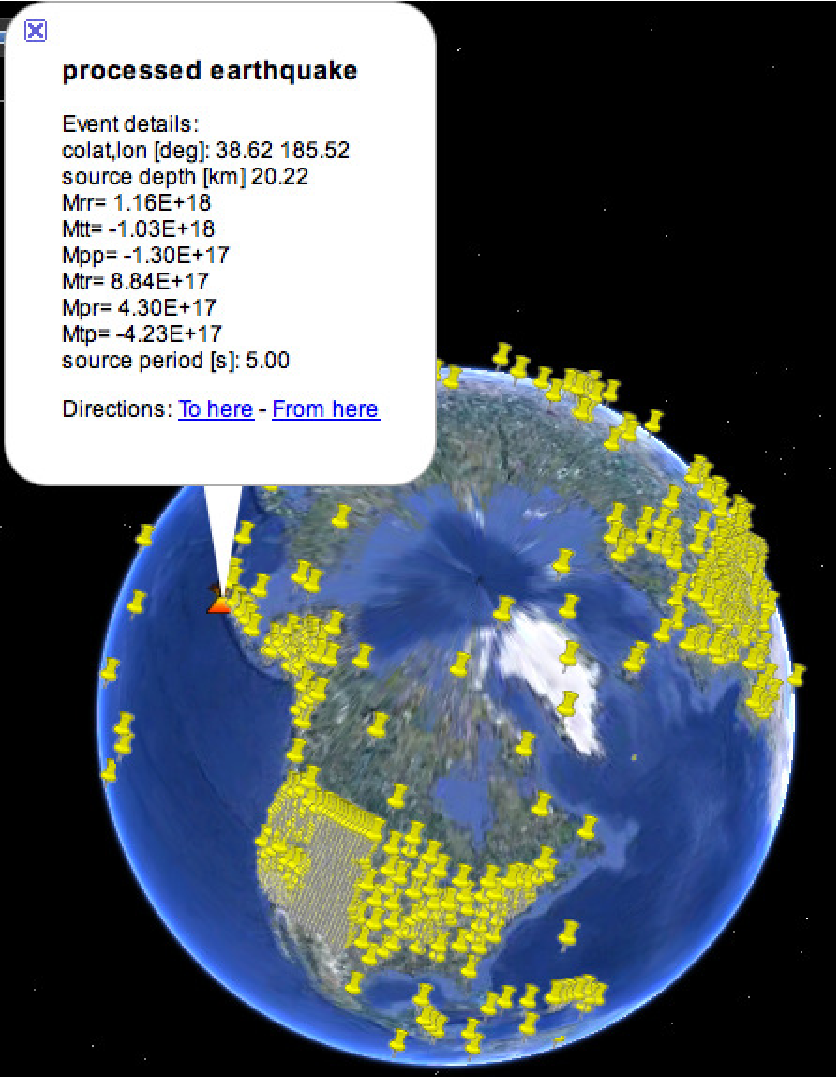
\includegraphics[scale=0.65]{googleearth_src_rec.pdf}
%         \caption{\textit{The kml file output from post processing. It contains
%         the rotated, original source-receiver geometry. Mouse-clicks on
%         earthquake location provide source information, mouse-clicks on
%         receiver pins receiver location information and graphics of the local
%         seismograms.}}
%     \end{center}
% \end{figure*}
% 
% \noindent \textbf{Wavefield snapshots in 3D}.\\
% The resultant vtk files are saved into {\tt
% Data\_Postprocessing/SNAPS/snap*vtk} and can be animated to a movie with
% paraview. Each processor dumps its own file.\\
% % 
% % % TODO ???
% % \noindent \textbf{We have tested:}\\
% % - rotations from cylindrical to spherical both in the solver and post processing\\
% % - moment tensor summation to explosion source using moment versus direct inclusion in solver\\
% % - compatibility of the two source and receiver file types (including cross-usage)\\
% % - summation of wavefield snapshots\\
% % - post processed convolution versus bandlimited stf in solver\\
% % 
% % \noindent \textbf{To Do}:\\
% % - turn strain wavefields into frequency domain for kerner\\
% % - rewrite scripts in Python\\
% % - parallelize snapshot creation\\
% % - netcdf seismogram databases
% % 
% % % TODO ?????
% % \section{Example workflows}
% % - this is under construction, but in directory EXAMPLES, you'll find
% % the input files for normal-mode summation code Mineos
% % (geodynamics.org), against which we have performed some
% % benchmarks. Caution: We have not managed to create a mode catalog that
% % is complete, in other words the reference solution is not to be seen
% % as precise in a quantitative way. Some pdfs in the directory show our
% % fit. It is useful to re-run such tests when first using AXISEM.
% 
% % %\newpage
% % \section{Kernel calculations}
% % Not included yet at this point... stay tuned!\\
% 
% % \noindent The philosophy of this 'scattering-integral' approach to sensitivity kernels 
% % is a once-and-for-all calculation of a database for a given background model,
% % i.e. including all potential earthquake depths. Everything else related to 
% % data, measurements, inversion parameters and observables, time windows, etc 
% % is done at the stage of inversion. At this time, output is limited to 
% % saving snapshots of the entire 2D mesh or a (contiguous) selection of grid points 
% % within elements. Under development is a more 
% % sophisticated method to either sample more sparsely, output into a wavelet 
% % basis, and straight into frequency domain. 
% 
% % In addition to using such sensitivity kernels for inversions, 
% % these can be used for Born modeling such that for any given 3D tomographic earth model, 
% % it is only a matter of a volumetric integration to determine the seismogram upon such tomographic 
% % models. This is not done yet either.
% 
% % \subsection{Kerner installation and compilation}
% % \subsection{Running the Kerner}
% % \subsection{Kerner input}
% % \subsection{Kerner computational aspects}
% % \subsection{Kerner code structure}
% % \subsection{Kerner output}
% % \subsection{Kerner post-processing}
% % \subsection{Kerner To Do}
% \newpage
% 
% % TODO merge todo lists!!!
% 
% 
% \section{To Do General}
% \subsection{Mesher}
% 
% \textbf{Top priority:} netcdf databases\\
% 
% \noindent\textbf{Medium priority:} Bending elements for sharp lateral discontinuities\\
% 
% \noindent\textbf{Low priority:} ellipticity, strongly deformed sphere
% (exostars)
% 
% \subsection{Solver}
% \noindent\textbf{Top priority:} 
% \begin{itemize}
%     \item benchmark heterogeneities
%     \item finite faults, multiple source simulations (4 Mij,
%     multiple depths, sequential and parallel)
%     \item dump fields in theta slices, dump fields in frequency domain,
%       netcdf, compression
%     \item Link input to NDLB
% \end{itemize}
% 
% \noindent\textbf{Medium priority:}
% \begin{itemize}
%     \item Oceans, fluid sphere (surface boundary condition),
%       inner-core anisotropy
%     \item GPU version, local high-order timestepping
%     \item Incorporate boundary-kernel dumps
%     \item non-blocking MPI, parallelization benchmark
% 
% \end{itemize}
% 
% \noindent\textbf{Low priority:}
% Gravity, python rewrite of submit.csh
% 
% \subsection{Post-processing}
% \noindent\textbf{Top priority:} 
% \begin{itemize}
%     \item Benchmark snapshot movies
%     \item Resampling of timeseries
%     \item rewrite wavefields in frequency domain
%     \item finite fault summation
%     \item extraction from synthetics database (VERCE, IRIS)
%     \item netcdf, streamline input
% \end{itemize}
% 
% \noindent\textbf{Medium priority:}
% Parallelize snapshot dumps (and other operations)\\
% 
% \noindent\textbf{Low priority:} python version

\section{References}

\noindent \textbf{Directly dealing with this code:}\vspace*{0.2cm}\\

(1) Tarje Nissen-Meyer, M. van Driel, S. St\"ahler, K. Hosseini,
S. Hempel, A. Fournier \textit{AxiSEM: Simulating high-frequency viscoelastic 3D global
wavefields}, to be submitted.\\

(2) Tarje Nissen-Meyer, F. A. Dahlen, A. Fournier (2007),
\textit{Spherical-earth Fr\'{e}chet sensitivity kernels},        
Geophysical Journal International 168(3),1051-1066. 
doi:10.1111/j.1365-246X.2006.03123.x                \\
                                                        
(3) Tarje Nissen-Meyer, A. Fournier, F. A. Dahlen (2007), 
\textit{A two-dimensional spectral-element method for
spherical-earth seismograms-I. Moment-tensor source}, 
Geophysical Journal International 168(3), 1067-1092. 
doi:10.1111/j.1365-246X.2006.03121.x                 \\
                                                       
(4) Tarje Nissen-Meyer, A. Fournier, F. A. Dahlen (2008),  
\textit{A two-dimensional spectral-element method for   
spherical-earth seismograms - II. Waves in solid-fluid media},
Geophysical Journal International, 174(3), 873-888.
doi:10.1111/j.1365-246X.2008.03813.x\\

(5) Tarje Nissen-Meyer (2007),
\textit{Full-wave seismic sensitivity in a spherical Earth},
Ph.D. thesis, Princeton University
(This includes refs (1)-(3) and more details.)\\
% 
% (5) Jean-Paul Ampuero, Tarje Nissen-Meyer (2011),
% \textit{High-order conservative time schemes in spectral-element methods 
% for seismic wave propagation.}, To be submitted to Geophys. J. Int.\\

%\noindent \textbf{NOTE:} Most important sections of these papers are in the Theory section below.\\

\noindent \textbf{Other references:}\vspace*{0.2cm}

(6) Deville, M. O., Fischer, P. F., Mund, E. H. (2002), 
\textit{High-Order Methods for Incompressible Fluid Flow}, 
Vol. 2, Cambridge monographs on Sppl. \& Comp. Math., Cambridge University Press.\\

(7) Tufo, H. M., Fischer, P. F. (2001), \textit{Fast Parallel Direct Solvers For Coarse Grid Problems}, 
61, 151-177, J. Par. and Dist. Comput.\\

(8) Bernardi, C., Dauge, M., Maday, Y. (1999), \textit{Spectral Methods for Axisymmetric Domains}, 
Vol. 3, Series in Appl. Math., Gauthier-Villars, Paris.\\

(9) Chaljub, E. (2000), \textit{Mod{\'{e}}lisation num{\'{e}}rique de la 
propagation d'ondes sismiques en g{\'{e}}om{\'{e}}trie sph{\'{e}}rique:
Application {\`{a}} la sismologie globale}, 
Ph.D. thesis, Universit{\'{e}} de Paris 7.\\

(10) Komatitsch D., Tromp, J. (2002), \textit{Spectral-element simulations of
global seismic wave propagation---I. Validation},
149, 390-412, Geophys. J. Int.


\end{document}
